%
% Master thesis template for Ghent University (2018)
%
%
%  !!!!!!!!!!!!!!!!!!!!!!!!!!!!!!!!!!!!!!!!!!!!!!!!!!!!!!!!!!!!
%  !!  MAKE SURE TO SET lualatex OR xelatex AS LATEX ENGINE  !!
%  !!!!!!!!!!!!!!!!!!!!!!!!!!!!!!!!!!!!!!!!!!!!!!!!!!!!!!!!!!!!
%  !! For overleaf:                                          !!
%  !!     1. click gear icon in top right                    !!
%  !!     2. select `lualatex` in "latex engine"             !!
%  !!     3. click "save project settings"                   !!
%  !!                                                        !!
%  !!!!!!!!!!!!!!!!!!!!!!!!!!!!!!!!!!!!!!!!!!!!!!!!!!!!!!!!!!!!
%
%
%  History
%    2014         Doctoral Thesis of Bruno Volckaert
%    2017         Adapted to master thesis by Jerico Moeyersons
%    2018         Cleanup by Merlijn Sebrechts
%
%  Latest version
%    https://github.com/galgalesh/masterproef-template
%
\documentclass[11pt,a4paper,twoside, openany]{book}
\usepackage[a4paper,includeheadfoot,margin=2.50cm]{geometry}

\setlength{\parindent}{0cm}           % indent of the first sentence of a paragraph
\setlength{\parskip}{1em}             % space between paragraphs
\renewcommand{\baselinestretch}{1.2}  % stretch horizontal space between everything

\usepackage{graphicx}
\graphicspath{{images/}}
\usepackage{pdfpages}
\usepackage{enumitem}
\usepackage{float}
\usepackage{caption}
\usepackage{subcaption}
\usepackage[toc,page]{appendix}

\usepackage{minted}                                    % for modern code highlighting
\newenvironment{code}{\captionsetup{type=listing}}{}   % To get multiline code fragments working: https://tex.stackexchange.com/a/53540/72273

\PassOptionsToPackage{hyphens}{url}
\usepackage{hyperref}
\usepackage{url}

\usepackage{quotchap}              % For the fancy quotes next to the chapter titles

\usepackage[numbers]{natbib}       % For bibliography; use numeric citations
\bibliographystyle{IEEEtran}
\usepackage[nottoc]{tocbibind}     % Put Bibliography in ToC

%
% Defines \checkmark to draw a checkmark
%
\usepackage{tikz}
\def\checkmark{\tikz\fill[scale=0.4](0,.35) -- (.25,0) -- (1,.7) -- (.25,.15) -- cycle;}

%
% For tables
%
\usepackage{booktabs}
\usepackage{array}
\usepackage{ragged2e}  % for '\RaggedRight' macro (allows hyphenation)
\newcolumntype{L}[1]{>{\raggedright\let\newline\\\arraybackslash\hspace{0pt}}m{#1}}
\newcolumntype{C}[1]{>{\centering\let\newline\\\arraybackslash\hspace{0pt}}m{#1}}
\newcolumntype{R}[1]{>{\raggedleft\let\newline\\\arraybackslash\hspace{0pt}}m{#1}}

%
% Support for splitting Dutch words correctly
%
\usepackage{polyglossia}
\setdefaultlanguage[babelshorthands=true]{dutch}

% Manually specify additional hypnations for words
\hyphenation{ten-ants appli-caties Open-Stack-Emu cloud-besturings-sys-temen besturings-sys-temen Dev-Stack Volckaert}

%
% Translated strings. If these aren't set, the English words are used.
%
\addto\captionsenglish{%
  \renewcommand{\contentsname}%
    {Inhoudsopgave}%
}
\renewcommand\appendixtocname{Bijlagen}
\renewcommand\appendixpagename{Bijlagen}
\renewcommand{\listoflistingscaption}{Lijst van listings}

%
% Set the title and your name
%
\title{Evaluatie van resource-allocatieschema's op OpenStack}
\author{Jerico Moeyersons}

%
%  END OF HEADER
%  The actual latex document content starts here.
%
\begin{document}






%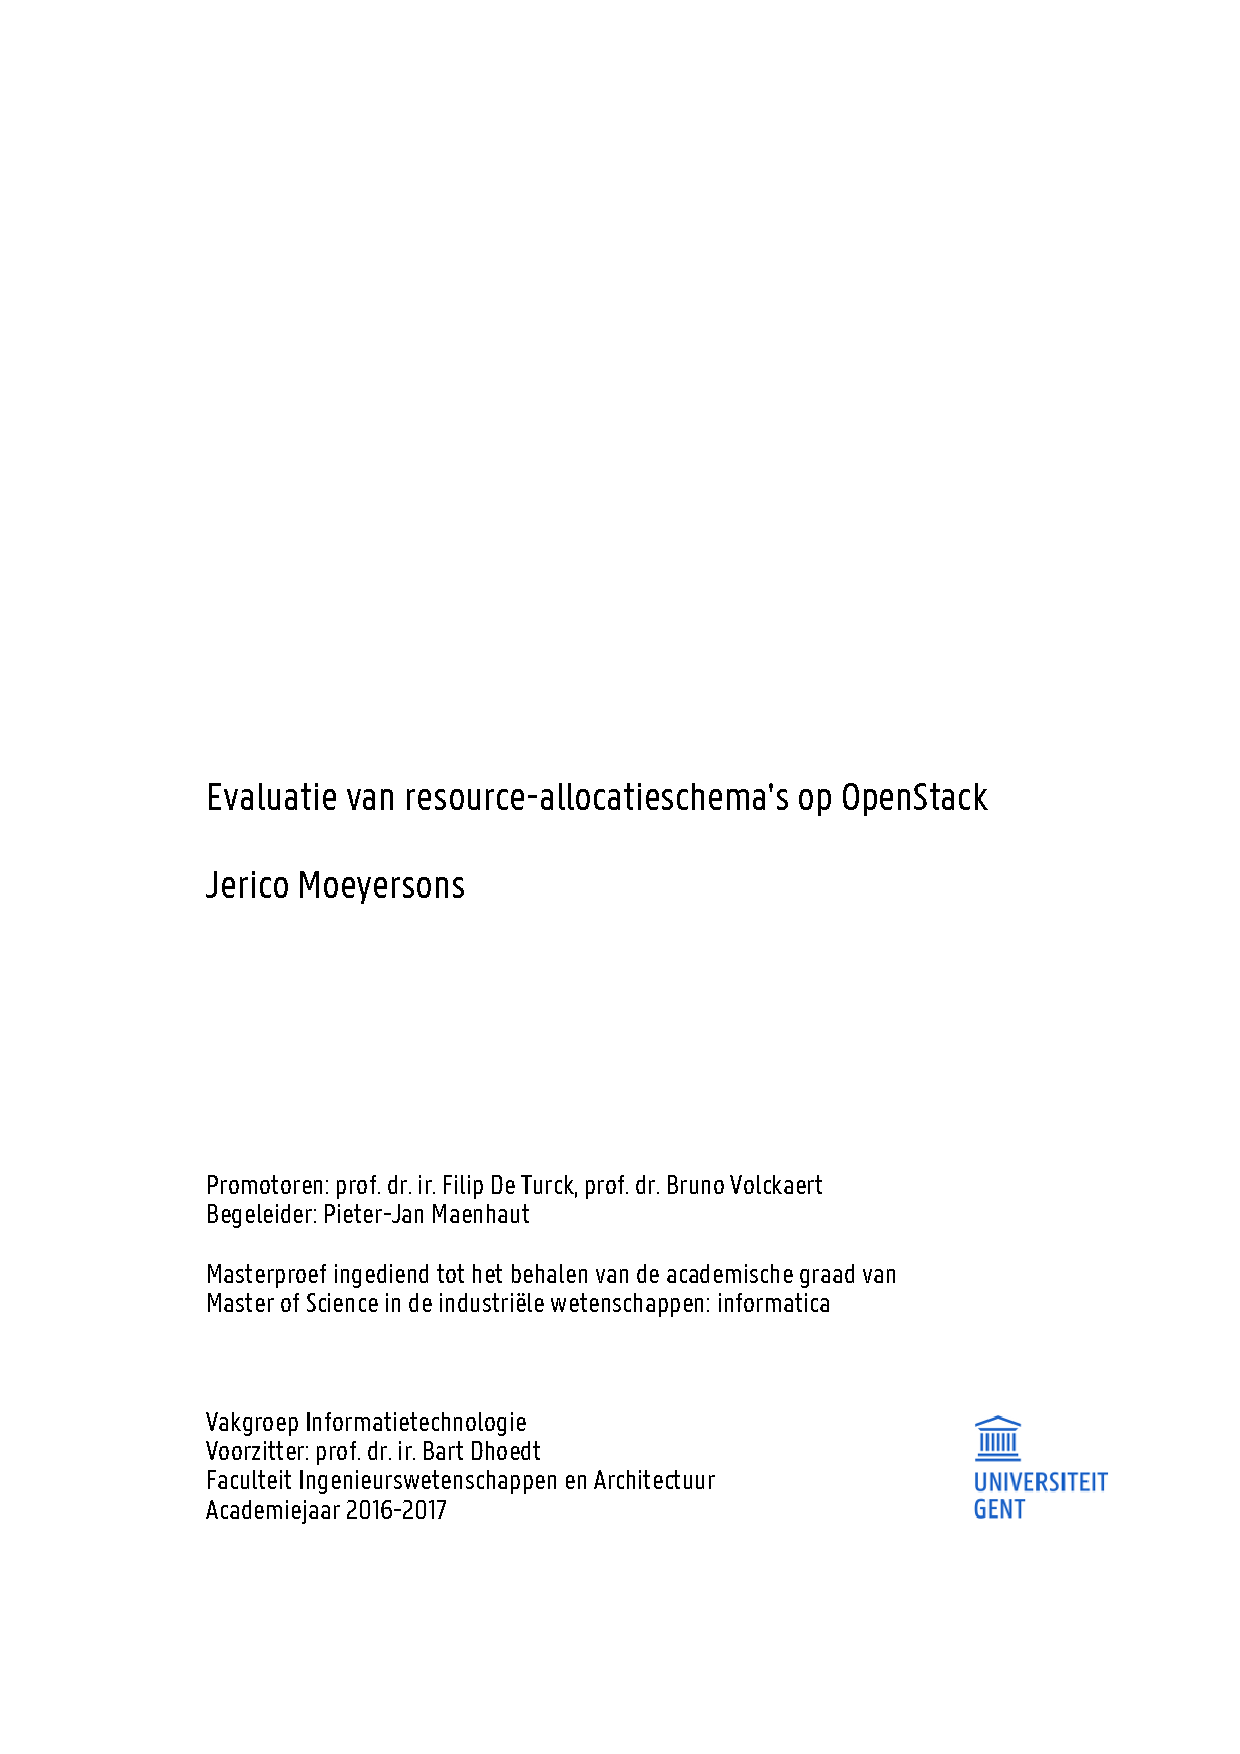
\includepdf{voorblad.pdf}             % Front matter
%\newpage\thispagestyle{empty}\mbox{}  % White page
%\thispagestyle{empty}    % Don't show page number

\begin{center}
\textbf{Dankwoord}
\end{center}

Na een intensieve periode van vijf maanden heb ik de laatste hand gelegd aan deze masterproef. Op verschillende vlakken heb ik nieuwe elementen binnen de wondere wereld van de informatica kunnen ontdekken. Daarom wil ik aan een aantal personen een welgemeende dankjewel zeggen om mij steeds te steunen tijdens het maken van deze masterproef.\\

Allereerst wil ik mijn promotoren, prof. dr. ir. Filip De Turck en prof. dr. Bruno Volckaert, bedanken voor het vertrouwen, de steun, de tips en de feedback. Ook mijn begeleider, de heer Pieter-Jan Maenhaut wil ik hartelijk bedanken voor de steun, de vele tips en uitgebreide feedback. Daarnaast wil ik ook mevrouw Leen Pollefliet bedanken voor de vele tips die ik nuttig heb kunnen gebruiken tijdens het schrijven en presenteren van deze masterproef. Vervolgens wil ik ook mijn vriendin, Lynn Haentjens, hartelijk bedanken om mij steeds te steunen in deze periode alsook voor het leveren van grammaticale feedback. Ten slotte wil ik ook mijn ouders bedanken voor de geleverde steun tijdens deze periode.\\

Om te eindigen met mijn dankwoord wil ik ook nog een aantal vrienden, namelijk Cédric Reyniers, Maxim Ronsse en Simon Vermeersch, bedanken voor de aangename middagpauzes, de relevante en ook de minder relevante gesprekken.\\
\\
Bedankt allemaal!\\
Jerico Moeyersons          % Word of thanks
%\newpage\thispagestyle{empty}\mbox{}  % White page
%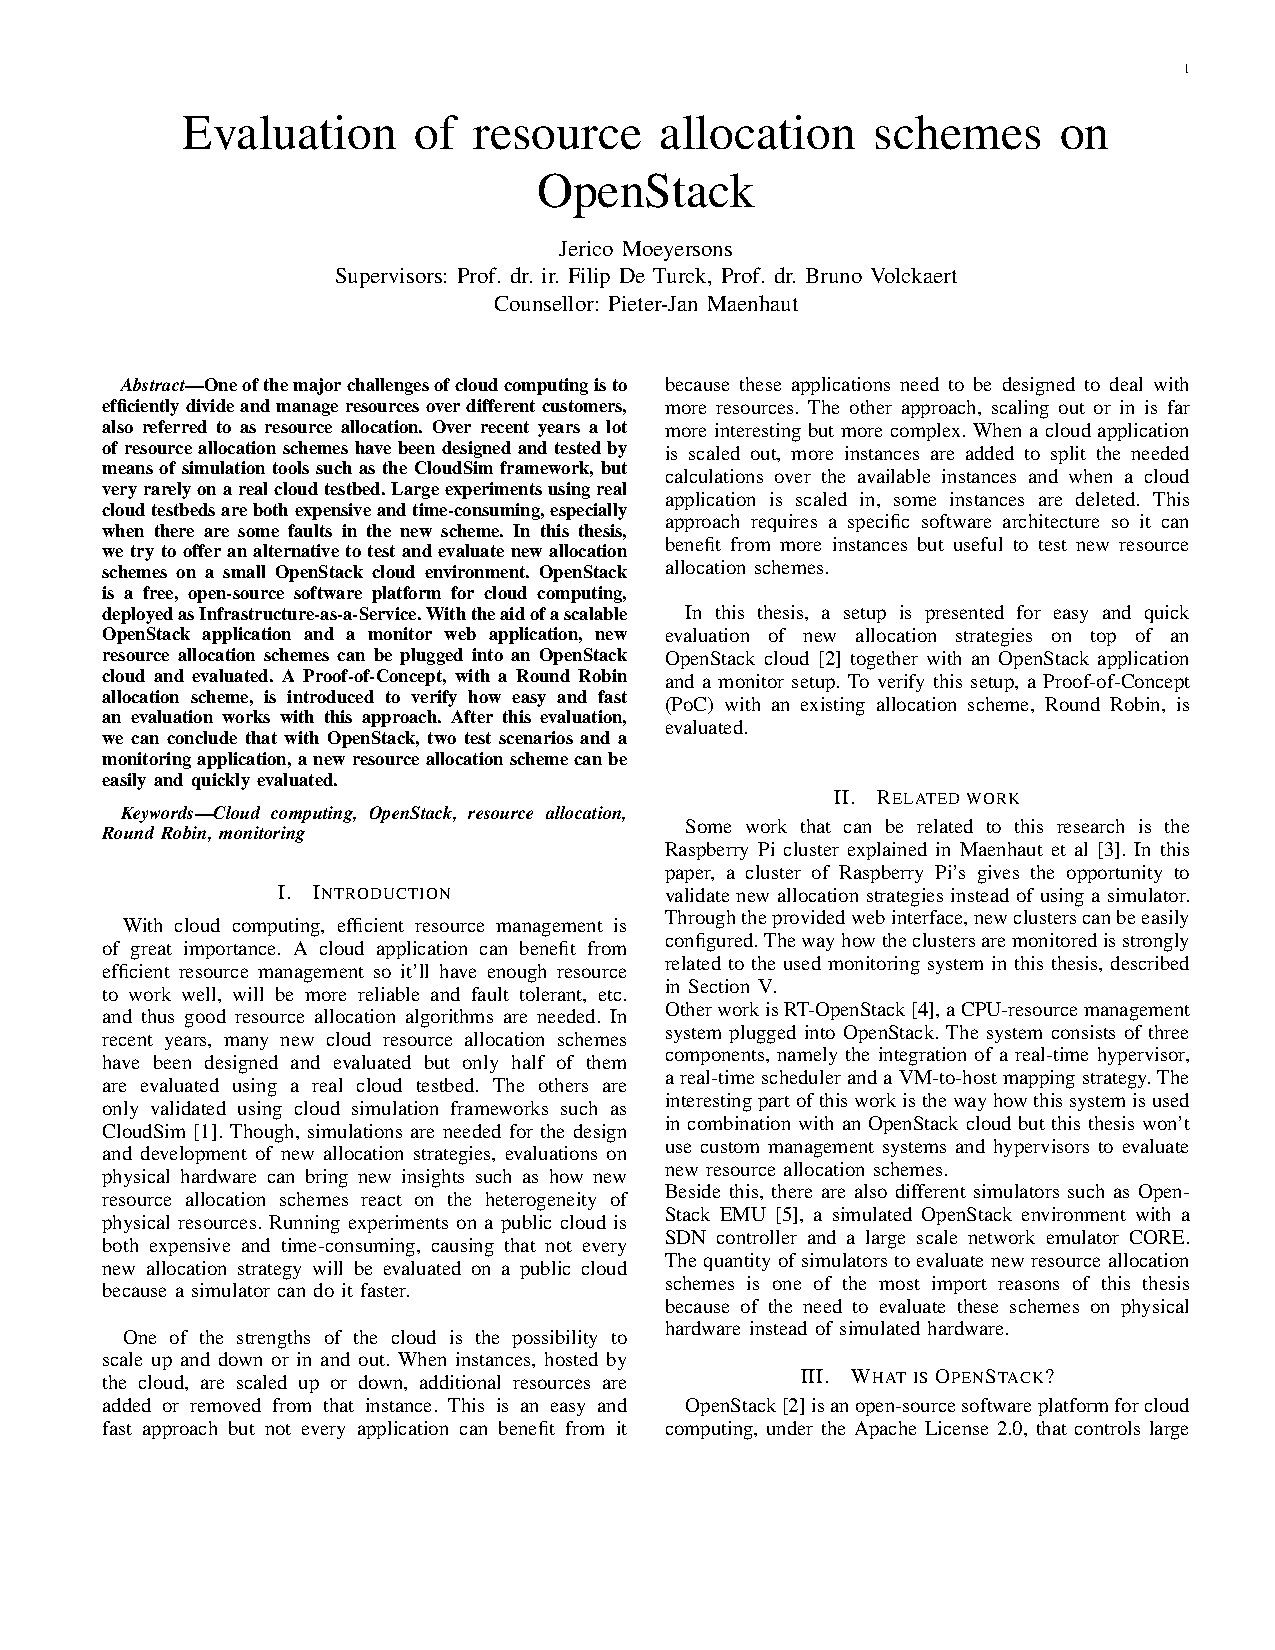
\includepdf[pages={-}]{abstract.pdf}  % Extended Abstract
\tableofcontents                      % Table of Contents
\listoffigures                        % List of figures
\listoftables                         % List of tables
\listoflistings                       % List of listings (code fragments)

%
% Include the main chapters of the thesis below
%
% Inspirerende caption 
%
%\begin{savequote}[0.55\linewidth]
%	``If you think you've seen this movie before, you are right. Cloud computing is based on the time-sharing model we leveraged years ago before we could afford our own computers. The idea is to share computing power among many companies and people, thereby reducing the cost of that computing power to those who leverage it. The value of time share and the core value of cloud computing are pretty much the same, only the resources these days are much better and more cost effective.''
%	\qauthor{\textasciitilde David Linthicum, author of Cloud Computing and SOA Convergence in Your Enterprise: A Step-by-Step Guide}
%\end{savequote}

\chapter{Introduction}
\label{chap:intro}

\section{Outline of the issue} %1p
\label{sec:issue}



% inspiratie kan je hier ook nog vinden:
% PREDICTION AND COMPARISON OF DOWNLINK ELECTRICFIELDAND UPLINK LOCALISED SARVALUES FOR REALISTIC INDOORWIRELESS PLANNING
Society is constantly getting more and more dependent on electronic communication. On any given moment in any given location, an electronic device
can request to connect to the bigger wireless network. Devices need more then ever to be connected, starting from small IOT sensors up to self-driving cars
which needs to be supported by the existing infrastructure. 

Once again it becomes clear why we're on the eve of a new generation of cellular communication named 5G. 
This new technology is capable of handling millions of connections every square meter %to do: klopt deze hoeveelheid want lijkt wel heel veel.
while satisfying only a few microseconds of a delay and providing connections up to 10Gbps \cite{5GFeatures}.

Also in exceptional and possibly life-threatening situations, we rely on the cellular network. For example during the terrorist attacks in Zaventem, a Belgian city.
Mobile network operators saw all telecommunications drastically increasing causing moments of contention. Some operators decided to temporarily exceed the exposure limits in
order to handle all connections. \cite{baseZaventem}

Electromagnetic exposure can however not be neglected. Research shows how exesive electromagnetic radiation can cause diverse biological side effects \cite{bioeffects}.
Because of public concern, the World Health Organization had launched a large, multidisciplinary research effort which eventually concluded that there was no sufficient evidence that confirmed 
that exposure to low level electromagnetic fields harmfull is \cite{WHO}. Nevertheless remains the public very concerned about potetial health risks.

\section{Objective}
\label{sec:objective}

In this master dissertation the electromagnetic exposure of  a user is investigated taking all prominent sources into account which include the user's own mobile device, basestations
and other users their \gls{UE}.

In order to determine the magnitude of exposure to which users in a certain area are exposed, various values need to be known. 
Not only the used technology but also the position of users and basestations need to be known. 
To make this research possible, an existing planning tool is used which gives insight in users and basestation distributions. Bitrates of idividual users, power useage of 
the different electronical devices and which basestations handels which users. The tool describes in other words a fully configured network.
In this way, all needed parameters will be known.

The electromagnetic exposure will then be analysed by applieing the tool in different scenarios. During the simulations
it is investigated how various input variables influence the network.

The calculation of electromagnic exposure originating from base stations is discussed in variously discussed in litterture. Papers who convert electromagnetic exposure
 into a single value is rather limited.
Not only how electromagnetic exposure behaves but also related values like power consumption or even coverage.



\textbf{research question 1:} How can a \gls{UABS} network be optimized to minimize global exposure and overal power consumption? What are the effects on the network?\\

\textbf{research question 2:} What are the advantages and disadvantages of a model as described in research question 1 compared the the already existing pahtloss oriented model.\\

\textbf{research question 3:} How does the \gls{UABS} fly height influence uplink and downlink exposure?


%todo: onderstaande tekst (in commentaar) is een letterlijke copy van J10-RDP. Het is hier gezet als referentie. Moet nog correct verwoorden:
%In this paper, prediction algorithms are created to
%simulate and visualise electric-field strengths due to
%downlink traffic and localised SARvalues due to uplink
%traffic. Downlink exposure are expressed in terms of
%whole-body exposure due to the electric-fields E originating
%from the base stations or APs, whereas uplink
%exposure are expressed in terms of localised SAR10g
%[SAR in 10 g of tissue(8)] values due to the mobile
%device’s transmitted signal. To

\section{Structure}
\label{sec:structure}

TODO: update this section

The following chapter \ref{chap:stateoftheart} exists of several succesive sections explaining how the electromagnetic exposure of a single human being is calculated. The first section \ref{sec:calculatingexposure}
explains how the exposure is calculated between a user and a single femtocell. Section \ref{sec:combiningexposure}  defines how to combine all exposures from the different femtocells towards a single users.
Finaly, section \ref{sec:radiationpatterns} explains how directional antenna's are taken into account.


\chapter{State of the art}
\label{chap:stateoftheart}

\section{Deployment tool for an UAV network}
\label{sec:stateoftheart:deploymenttool}

Calculating electromagnetic exposure requires knowledge about the area. The position of base stations need to be know,
 the transmission power used by the antenna and how far is the user separated from this base stations are only a few parameters
 that have to be considered.

The WAVES research group at UGent has developed a deployment tool for disaster scenarios with the aid of UAVs \cite{J2}.
The idea of this  UAV-aided emergency network is that in case of a disaster, the existing network might be damaged and won't be able 
to handle all users who are trying to reconnect to the backbone network. 
The tool makes a fast deployable network possible by attaching femtocells to UAVs, so-called \gls{UABS}s.
The tool will orchestrate the \gls{UABS}s over the disaster area. This tool is thus a suitable starting point and works as follows:

%The optimal placement for each \gls{UABS} needs to be defined to make sure that as many users as possible are properly reconnected to the backbone network while satisfying certain restrictions. 
%To make these calculations as realistic as possible the architecture of the several buildings present in the area is described in a shapefile. 
%A deployment tool calculates the optimal position of the \gls{UABS} by taking the 3D models of the building into account along with some femtocell specifications and user distribution. This deployment tool is developed by the WAVES research group, a department within Ghent University.

The deployment tool will try to calculate the optimal placement for each \gls{UABS} and requires therefore a description of the area where the UAV-aided network needs to 
be deployed. This is done with the use of so-called shape files. Theses files contains tree dimensional descriptions of the buildings present in the area and are
key values in approaching results as realistic as possible. Furthermore, the tool also requires a time period and a configuration file containing technical specifications of the type of \gls{UABS} that is being used. 
The tool will thereafter randomly distribute users over the area and assigns a certain bitrate to them. \\
\\
In a second phase, the optimal position for each \gls{UABS} is calculated. This is done by trying to locate a \gls{UABS} above each active user. Two options are possible.
If a flying height is defined, a base stations is placed above each user at the given height, unless a building is obstructing it's location. Then, no base station will be located above that user.
If no flying height is given to the tool, the base station is located 4 meters above the outdoor user or 4 meters above the building where the indoor user resides. 
The later is only allowed if the suggested height remains below the given maximum allowed height. \\
\\
Finally, all  \gls{UABS} are sorted on wether they were active or not, followed by the increasing pathloss from each \gls{UABS} to that user.
So the algorithm starts by checking for each active \gls{UABS} if it can cover the user. If this is the case, the user will be connected to this \gls{UABS}. If not,
the second active base station with a (slightly) worse pathloss is considered. If no active base station is suitable, inactive \gls{UABS} are considered. The user remains uncovered if no \gls{UABS}
is found. The reasoning behind first only considering base stations that are already active is the hight cost that comes along with each drone. \\
\\
Up till now, the tool has only calculated some suggestions. The effective provisioning is done in the fourth phase where drones are sorted by the ammount of users it covers. As long as \gls{UABS}
are available in the facility where they reside, \gls{UABS} are provisioned and its users are marked as covered.


\section{Electromagnetic exposure}

\subsection{Electromagnetic field radiation} % (fold)
\label{sub:emf}
People in a telecommunication network are exposed to far field electromagnetic radiation originating from base stations and other \gls{UE}. 
Network planners need to make sure that the the electromagnetic fields (expressed in V/m) does not exceed limitations enforced 
by the government. These limits are location dependent. The european union recommend the guidelines as defined by the \gls{ICNIRP} which limits electromagnetic exposure to 61 V/m.
Each european country needs to decide for themselves which limitations to enforce. Belgium for example delegated this responsibility to Flanders, Brussels and Wallonia \cite{J23}.

The used deployment tool is applied in Ghent, a Flemish city in Belgium. The standards defined by the Flemish government is therefore applicable.
They state that in the 2.6 Ghz frequency band, an individual antenna can't exceed 4.5 V/m and the cumulative sum of all fixed sources 31 V/m \cite{S13_normenBelgie}.

\subsection{Specific Absorption Rate}

\gls{SAR} represents the rate that electromagnetic energy is absorbed by human tissue with the thermal effect as it's most important health consequence.
The volume of this tissue is typically 1g or 10g. The Federal Communications Commission of the United States defines regulations based on 1g tissue (indicated as $SAR_{1g}$) 
while the European Union handles the 
10g model ($SAR_{10g}$). $SAR$ values can further be categorized based on the area it covers. 
A first one is whole body \gls{SAR} ($SAR^{wb}$) which is the average absorbed radiation over the entire 
body. The second type is more precisely. Localized \gls{SAR}-values cover only  a part of the human body like the head.
The \gls{ICNIRP} has concluded that the threshold effect for $SAR^{wb}_{10g}$ is at 4 W/kg meaning that any higher absorption rate would overwhelm the thermoregulatory capacity of the human body.
Whole body values between 1 and 4 W/kg increases the temperature of human body less then 1°C which is proven not to be harmful for a healthy human being\cite{J24}.
Thereafter, a safety margin is introduced to tackle unknown variables like experimental errors, increased sensitivity for certain population groups and so on. 
This results in a whole body $SAR_{10g}$ of $0.8 W/kg$ and $2 W/kg$ for localized $SAR_{10g}$ at head and torso area \cite{J23}.

%todo: de 10g slaat al op localized, vandaar dat het maar 10g is, anders is het whole-body
%todo: we kunnen niet sar10gmax gebruiken want This means that the SAR calculations will be worst-case and possibly an overestimation of the real localised SAR. (herwoorden voor plagiaat)
%Human exposure caused by downlink traffic is a not negligible asset. However, telecommunications is not a one-way street. When connecting to a UMTS network, also uplink data caused by the \gls{UE} should be considered.
%\gls{UE} generates, just like femtocells, electromagnetic waves to which a user is exposed. A part of this radiation goes to the femtocell, another part enters the body of its user. How much electormagnic strenghts enters the body is defined as \gls{SAR} and is measured with 10g biological tissue which represents the human skin. This value will from now on be expressed as $SAR_{10g}$. 
%A mobile device induces two types of exposure: local and whole-body. 

\subsection{Related work} % (fold)
\label{sub:general}
The goals of this master dissertation is the investigation of electromagnetic exposure considering all sources. Three types of sources are considered: electromagnetic radiation 
caused by basestations, near field radiation from the users own device and far field radiation originating from other users their equipment. This electromagnetic radiation is thereafter
absorbed by the human body which will be expressed in \gls{SAR} values.

Several papers exist calculating exposure originating from certain sources but very limited research has been done covering the whole picture.
In \cite{J6_originalExposureFormula} is described how electromagnetic radiation of several WiFi access points is being calculated. The authors of \cite{J1} used this knowledge 
to investigate electrmangetic exposure originating from basestations in a more outdoor environment. \cite{J10_RDP, J10.1} addresses the fact that 
also \gls{UL} traffic from the user's device should be considered. They therefore investigated indoor exposure. They did not only consider the electromagnetic radiation
but also how much is absorbed by the body wich will be expressed as specific absorption rate. Since the authors only covered voice calls,
uplink SAR was expressed in localized SAR values while the downlink traffic is expressed in whole body SAR. With the advent of 5G, paper \cite{J17_kuehn2019modelling} has been 
published describing how localized SAR values are achieved from all sources. More precisly: all mobile phones and all basestations in the network after which they converted the electromagnetic 
exposure to localized SAR values.
Finally, \cite{J22_plets2015joint} describes how both \gls{UL} and \gls{DL} traffic can be converted in whole body SAR values making it possible to achieve an overall picture. They applied this formula 
however only for the user's own device.

In a realistic network like the used deployment tool, some users are calling while annother part is using other type of telecommunication services like browsing the web.
Therefore, all absorbed electromagnetic exposure should be expressend in whole body SAR while still covering all sources.

\section{Optimizing towards electromagnetic exposure and power consumption}
\gls{UABS}s are drones with femtocell base stations attached to it. Drones can remain in the air for only a limited time, which is certainly 
the  case when also an antenna needs to be connected to the battery of the its carrier. It is therefore
interesting to not only considering electromagnetic exposure of the user but also the power consumption that comes with it. 
However an increasing transmission powers of an antenna comes with an increasing electromagnetic exposure, this is not the case considering
both values for an entire network. In fact, the autors from \cite{J1}  prove that both become inversely equivelent.

If a network is optimized towards power consumption, less drones will be provisioned radiating at higher power levels. This is because not only 
the transmission power is considered but also the power needed to keep the drone in the air. Therefore, it is cheaper to cover a user by 
increasing the antenna's transmission power of an already activated drone nearby as it therefore prevents the power cost of a new drone.
By increasing the transmission power, also the electomagnetic exposure will increase for users closer to that drone. An exposure optimized
network will therefore faster decide to power up a new drone.

todo: geen grid maar per user--> methodology

\section{Technologies}
\subsection{Type of drone}

Section \ref{sec:stateoftheart:deploymenttool} describes how femtocell antennae will be connected to helicopter drones. Two types of 
drones are considered in \cite{J2}: an off-the-shelf drone affordable by the generic public and a more expensive drone. The results in \cite{J2}
show that the second type will require less drones to cover the same number of users and will last longer in the air. The research in this paper
will therefore be done with the usage of the second type. A technical overview of this drone is given in table \ref{table:dronespecs}.

\begin{table}[h!]
\centering
\begin{tabular}{|l|c|l|}
\hline
 parameter          & value         \\    \hline
 Carrier power      & 13.0 A \\
 average carrier speed           & 12.0 m/s       \\ 
 Average carrier power usage    & 17.33 Ah      \\ 
 Carrier battery voltage        & 22.2 V \\ \hline
\end{tabular}
\caption{specifications for the used drone.}
\label{table:dronespecs}
\end{table}

\subsection{LTE}
The tool make usage of \gls{LTE} which is by the general public better known as 4G which allows better \gls{UL} and \gls{DL} data speeds 
compared to its predecessors and is based on an all IP architecture. LTE can cover macrocells supporting cell sizes ranging from 5 km up to 100 km. 
These type of antennae are usually attached to transmission towers along highways or on top of buildings. LTE supports however also smaller cells like
femtocells covering only a few hundred meters. They are therefore more portable, require less energy and won't require a telecommunication operator because
of it's simplicity. Femtocell base stations are therefore used by the deployment tool.
Further, \gls{LTE} also support both \gls{FDD} and \gls{TDD}.

\gls{FDD} makes simultaneous \gls{UL} and \gls{DL} traffic possible by assiging different frequencies within the frequency range 
to both data streams. A small guardband is used between \gls{UL} and \gls{DL} directions in other to prevent interference.

\gls{TDD} allows  \gls{UL} and \gls{DL} by splitting the time domain. Meaning that both traffic directions use the same frequency and therefore
alternately (in time) use the frequency spectrum. A small time interval is used to prevent interference in case of a slightly bad timed synchronization.

This master dissertation will make usage of \gls{FDD}.

\subsection{Type of antenna} % (fold)

An important part of this master dissertation is the type of antenna that will be used by the femtocell base stations. The deployment tool makes use
of drones that will position the femtocell base stations in the right position.  Using conventional 
sector antennae, as used by traditional terrestrial transmission towers, would be to complicated for a simple drone. 
The characteristics of microstrip antennae will therefore be investigated.

Microtstrip antennae provide several advantages compared to traditional antennae \cite{J13_singh2011micro, J14_antennadesign}. Microstrip antennae
are lightweight, low in cost and thin causing them to be more aerodynamic which is  a useful feature since the antennae will be attached
to flying drones.

A basic microstrip antenna like figure \ref{fig:basicpatchantenna} consists out of a ground plane and
a radiating patch, both separated with a dielectric substrate. Several variations exist like microstrip patch antenna, microstrip slot antenna and printed dipole antenna which
has all similar characteristics. They are all thin, support dual frequency operation and they all have the disadvantage that they 
will transmit at frequencies outside the aimed band which is also known as
\gls{spuriousradiation}. The microstrip patch and slot antenna support both linear
and circular polarization while the printed dipole only support linear polarization. Further is the fabrication of a microstrip patch antenna considered to be the easiest of its competitors. 

\begin{figure}[H]
\centering
  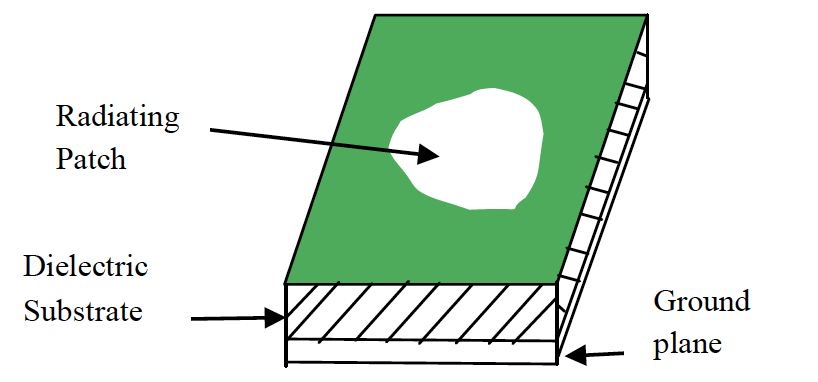
\includegraphics[width=\textwidth/2]{../images/patchantenna.png}
  \caption{General design of a microstrip antenna}
  \label{fig:basicpatchantenna}
\end{figure}

The microstrip antenna requires besides the groundplane, dielectric substrate and the radiation patch also a feed line. Several feeding techniques exists of which the most popular are: coaxial probe feeding, microstrip line and apeture coupling. %and Microstrip Patch Antenna
(todo: more refs? gebruik nummer twee van J13 (p2))

A first feeding method is with the usage of a coaxial cable where the outer conductor is attached to the ground plane and the inner conductor to the radiations patch. Modelling is however difficult, escpecially for thic substrates as will be used in this master dissertation.
A second option is the usage of a microstrip line. This type of feeding is much easier to model since the microstrip line can be seen as en extension of the radiating patch.
A disadvantage is the increased \gls{spuriousradiation} which limits bandwith.
A third is proximity coupling which has the largest bandwidth and low \gls{spuriousradiation}. It consist however of two dielectric substrates causing the overall thickness
of the antenna to increase as well as it's fabrication difficulty.
(todo: tekst te weinig, bespreek ook apperture coupled attenna (zelfde paper als de rest))

The increasing usage of the microstrip patch antennae can be explained by it's easy fabrication and lightweightness and therefore knows a widespread application in the millitary, global possitioning systems, telemedicine, WiMax applications and so on.
The authors of \cite{J13_microstripadvantages} also state that some of the disadvantages like lower gain and power handling can be solved with the usage of an array configuration.

The radiating patch is usually made of a thin layer of either gold or copper \cite{J14_antennadesign,J15_antennadesign}
and can be any form. However, shapes besides a circle or rectangle would require large numerical computation \cite{J14_antennadesign}.
A simple rectangular shape will thus be used.
Further is also the dielectric constant of the substrate important which typically varies between 2.2 and 12. Finding a good dielectric depends on how the antenna will used. A lower
dielectric constant with a thick substrate will result in better performance, better efficiency and larger bandwidths  \cite{J15_antennadesign}.
On the other hand, a larger dielectric constant reduce de dimensions of the antenna \cite{J14_antennadesign}
which is also useful when attaching the 
antenna to a limited surface. Glass as a dielectric substrate with a constant of 4.4 will therefore be used.
\chapter{Gerelateerd werk}
\label{chap:rel_work}

Aangezien resource allocatieschema's van clouds nog steeds worden onderzocht, bestaan er enkele werken die gerelateerd kunnen worden aan deze masterproef. In Sectie~\ref{sec:newcras} wordt nadien een overzicht gegeven van reeds ontwikkelde cloud resource allocatieschema's.

\section{Relevant onderzoek}
\label{sec:related_work}

Een zeer gerelateerd werk van Maenhaut et al.~\cite{Maenhaut2017} beschrijft een Raspberry Pi cluster voor het valideren van cloud management strategieën. Dankzij een eenvoudige webinterface kan in deze demo alles eenvoudig geconfigureerd en getest worden. De Node.js-agent beschreven in Sectie~\ref{sec:nodejs-agent} heeft dan ook inspiratie gehaald uit deze demo mits enkele aanpassingen en verbeteringen omdat hier gebruik wordt gemaakt van fysieke servers in plaats van Raspberry Pi clusters.

RT-OpenStack~\cite{Xi2015} plugt een CPU-resource management systeem in op een OpenStack omgeving. Het is een systeem bestaande uit 3 onderdelen, namelijk de integratie van een real-time hypervisor, een real-time scheduler en een VM-to-host mapping strategie wat dus vooral de nadruk legt op real-time VM's. Een belangrijke onderdeel van dat werk is de manier waarop RT-OpenStack werkt in combinatie met een normale OpenStack cloud-omgeving maar in deze thesis wordt er geen gebruik gemaakt van een aangepast management systeem noch van aangepaste hypervisors voor de evaluatie van allocatieschema's.

Een ander voorbeeld van een inplugbaar framework in OpenStack is OpenStack Neat~\cite{Beloglazov2014}.  OpenStack Neat is eenvoudig inplugbaar in een bestaande OpenStack cloud-omgeving en gaat zorgen voor dynamische en energie-efficiënte algoritmen om VM's te consolideren. Daarbovenop biedt het ook de mogelijkheid om nieuwe VM consolidering algoritmen te evalueren en te vergelijken. De structuur van het framework en de werking ervan zijn zeer relevant doch ligt in deze thesis de focus meer op de correcte werking van het algoritme in plaats van de energie-efficiëntie.

Daarnaast bestaan er ook verschillende simulators om nieuwe schema's te testen zoals bijvoorbeeld OpenStackEmu~\cite{Benet2017}. Hierbij wordt een OpenStack omgeving gesimuleerd samen met een \textit{Software Defined Networking (SDN)} controller en een large-scale network emulator CORE (\textit{Common Open Research Emulator}). Dergelijke oplossing benadert al iets meer een reëele cloud-omgeving en de gebruikte methode is gerelateerd aan de werking van deze thesis. Enkel wordt er hier getracht om een echte cloud-omgeving te gebruiken in plaats van te benaderen of te simuleren.

Een ander voorbeeld van een simulatietool wordt beschreven door Maenhaut et al.~\cite{Maenhaut2016} waarbij verschillende nieuwe schema's worden getest met behulp van verschillende invoerparameters. Deze resultaten geven een goed oog op de mogelijk performantie maar opnieuw gaat het om een simulator waarbij mogelijke constanten van een echte cloud-omgeving verborgen blijven. Deze thesis probeert daarom deze verborgen constanten zichtbaar te maken door de evaluatie uit te voeren op een reëel cloud-testbed.

Ten slotte bestaan er ook enkele interfaces om eenvoudig met OpenStack te communiceren zoals Apache Libcloud~\cite{Libcloud}, een python bibliotheek, of pkgcloud~\cite{pkgcloud}, een node.js-pakket. Via een eenvoudige interface bieden ze een mogelijkheid aan om met verschillende cloud-besturingssystemen, zoals onder andere OpenStack, Google Cloud Platform, CloudFlare, etc te communiceren en hierop commando's uit te voeren. Indien deze interfaces gebruikt kunnen worden bij bijvoorbeeld de evaluatie van zo'n nieuw schema kan dit de overstap naar een andere cloud-omgeving zeer eenvoudig maken aangezien de commando's dezelfde blijven en de interface deze automatisch zal omvormen naar de commando's typisch voor het gebruikte cloud-systeem. Deze bibliotheken bieden dus de mogelijkheid om gebruikte cloud-omgeving te besturen en niet om evaluaties uit te voeren.

\section{Beknopt overzicht van cloud resource allocatieschema's}
\label{sec:newcras}

Globale planning van gevirtualiseerde resources beschrijft het systeemwijde perspectief van de allocatie van fysieke en virtuele resources in een cloud omgeving. De meeste van deze methoden zijn gecentraliseerd zodat ze volledige controle hebben over de allocatie van een verkregen set van resources. De hiervoor gebruikte technieken worden onderverdeeld in 4 groepen namelijk de initiële plaatsing van de VM's, dynamische plaatsing van VM's, VM-plaatsing rekening houdend met de netwerkbronnen en technieken om het energieverbuik te minderen.

De initiële plaatsing van VM's op fysieke machine's is gerelateerd aan het \textit{vector bin packing} probleem, wat NP-hard is waardoor enkel heuristische methoden in aanmerking komen~\cite{Hochba1997}. Enkele voorbeelden hiervan zijn de \textit{First Fit Decreasing (FFD)} en \textit{Best Fit Decreasing} heuristieken die gebaseerd zijn op gulzige algoritmen~\cite{Panigrahy2011} of het \textit{Reordering Grouping Algorithm (RGGA)} gebaseerd op genetische algoritmen~\cite{Wilcox2011}. Daarnaast zijn er ook algoritmen om dynamisch een pool van resources te alloceren aan een set van concurrerende VM's en algoritmen die rekening houden met beperkingen opgelegd door de cloud-gebruikers.\\
\textit{Live migration}~\cite{Clark2005} of dynamische plaatsing van virtuele machines is een zeer handige techniek waarbij een draaiende VM wordt gepauzeerd, geserialiseerd en verplaatst naar een andere fysieke machine. Gebruikte heuristieken hiervoor zijn bijvoorbeeld de \textit{first-fit} heuristiek~\cite{Bobroff2007} dat de verschillende VM's dynamisch hermapt op de fysieke machine's met als resultaat een minimaal gebruik van fysieke machines, of \textit{King-fisher}~\cite{Sharma2011}, een set van technieken voor VM-schaling, replicatie en migratie waarbij de problemen worden geformuleerd als ILP-model. Een ander voorbeeld is het live migration proces voorstellen als een roman zodat het probleem herleid wordt tot een \textit{Stable Marriage} probleem~\cite{Xu2011}.

Er zijn ook algoritmen die rekening houden met de netwerktopologie vooraleer een VM wordt geplaatst op een fysieke machine. Een voorbeeld hiervan zijn heuristieken die VM's die data-intensief met elkaar moeten communiceren dicht bij elkaar trachten te plaatsen.

Technieken om het energieverbuik te minderen zijn gebaseerd op \textit{right-sizing} van datacenters.\footnote{Het dynamisch herschalen van actieve fysieke nodes bij een veranderende werklast.}~\cite{Chase2001} Nieuwere methoden maken een combinatie van deze technieken om het energieverbuik te minderen samen met de mogelijkheid tot het aanpassen van de processorsnelheid van fysieke nodes met behulp van \textit{Dynamic Voltage Scaling} (DVS). Dit zorgt ervoor dat de kloksnelheid van een processor kan dalen (minder stroomverbruik) en een processor kan werken in een omgeving met hogere temperaturen (minder koeling) wat in beide gevallen zorgt voor een lagere energieconsumptie.

Naast de globale planning van gevirtualiseerde resources moet er ook lokale planning van de gevirtualiseerde resources gebeuren. Lokaal resource management bepaalt hoe de fysieke resources worden gedeeld tussen de gevirtualiseerde resources die erop draaien. Recente onderzoeken proberen hiervoor een volledige automatische oplossing te vinden die constant de VM's monitort waarbij dynamisch extra resources voorzien worden, rekening houdend met de afgesloten SLA's. Technieken die hiervoor gebruikt worden zijn onder andere \textit{fuzzy-logic}~\cite{Xu2008} en \textit{reinforcement learning}~\cite{Rao2011}. Een voorbeeld van een systeem dat het delen van lokale fysieke resources tussen virtuele resources vergemakkelijkt is \textit{DeepDive}~\cite{Novakovic2013}, een systeem ontwikkeld om interferentie tussen verschillende VM's te identificeren en te verzachten.

\begin{table}[tbp]
	\centering
	\captionsetup{justification=centering}
	\caption[Overzicht resource-allocatieschema's]{Overzicht resource-allocatieschema's \\
		A=Algoritme, P=Protocol, F=Framework S=Simulator, C=Cloud, ILP=Integer Linair Programming, GH = Greedy Heuristic, SBP=Stochastic Bin Packing, MINLP=Particle swarm, RR=Round-Robin, SA=Simulated Annealing, SMT=Satisfiabilty Module Theory, FFD=First Fit Decreasing, MI(N)=Mixed Integer (Non-), SPLE=Software Product Line Engineering, L=Lijst, G=Graaf, B=Boom, FN=Fysieke node, Mig=Migraties, (?)=Niet vermeld}
	\label{tab:resallocschemes}
	\resizebox{\textwidth}{!}{%
	\begin{tabular}{L{4cm} l C{2cm} c c c c}
		\toprule
		Naam & Jaar & Type  & A | F | P  & Invoer & Uitvoer & Getest  \\ \midrule
		Alicherry et al.~\cite{Alicherry2012} & 2012 & k-sneden & A & G & par\{G\} & S \\
		MCRVMP~\cite{Biran2012} & 2012 & ILP \& GH & A & B\{netwerk\} & VM-plaatsing & C\\
		Breitgand et al.~\cite{Breitgand2012} & 2012 & SBP & A & L\{VM\} & L\{VM\}/Bin & S \\
		Snooze~\cite{Feller2012} & 2012 & Framework & F & - & - & C \\
		Sequence planning~\cite{Ghorbani2012} & 2012 & Heuristiek & A & Net + S\{Mig\} & L\{VM/Mig\} & S \\
		Giurgu et al.~\cite{Giurgiu2012} & 2012 & Beam seach & A &- & VNI-plaatsing & S \\
		Seagull~\cite{Guo2012} & 2012 & Framework & F & - & - & C \\
		v-Bundle~\cite{Hu2012} & 2012 & Novel & A & B\{Node\} & VM-plaatsing & S + C \\
		VMPR~\cite{Jiang2012} & 2012 & Markov-ketens & A & L\{Jobs\} & Job-afhandeling & S (?) \\
		TROPIC~\cite{Liu2012} & 2012 & Framework & F & - & - & C \\
		Konstanteli et al.~\cite{Konstanteli2012} & 2012 & MINLP & A & - & Gealloceerde resources & C \\
		CloudMap~\cite{Viswanathan2012} & 2012 & RR & A & Resource-verbruik & Servercluster & C \\
		VirtualKnotter~\cite{Zou2014} & 2012 & SA & A & Verkeer & VM-plaatsing & S \\
		P*~\cite{Wuhib2012a} & 2012 & Gossip protocol & P & - & - & S \\
		Scattered~\cite{Zhang2016} & 2012 & Black- en Gray-box & A & L\{hosts\} & VM-plaatsing & C \\
		VMM-Planner~\cite{Al-haj2013} & 2013 & SMT & A & VM-plaatsing + doel & L\{Mig\} & C \\
		Shi et al.~\cite{Shi2013} & 2013 & ILP & A & L\{FN\} & VM-plaatsing & C \\
		Shi et al.~\cite{Shi2013} & 2013 & FFD & A & L\{FN\} & VM-plaatsing & C \\
		Omega~\cite{Schwarzkopf2013} & 2013 & Large scale & F & - & - & S \\
		PACMan~\cite{Nath2013} & 2013 & - & A & VM interferentie & VM-plaatsing & C \\
		Max-BRU~\cite{NguyenTrungHieu2014} & 2014 & - & A & Datacenter & VM-allocatie & C \\
		RT-OpenStack~\cite{Xi2015} & 2015 & - & A & Budget VCPU's & CPU-resources & C \\
		J.Bi et al.~\cite{Bi2015} & 2015 & SA, MINLP & A & Datacenter & VM-allocatie & S \\
		F. Fakhfakh et al.~\cite{Fakhfakh2015} & 2015 & MILP & A & L\{Taken, deadl.\} & VM-allocatie & S \\
		L. Li et al.~\cite{Li2015} & 2015 & Framework & F & - & - & (C) \\
		A. Ruiz-Alvarez et al.~\cite{Ruiz-Alvarez2015} & 2015 & IPL & A & Max. duur & Optimale kost & C \\
		Dohko~\cite{Leite2015} & 2015 & SPLE & A & Vereisten & Resource selectie & S \\
		A.aral et al.~\cite{Aral2015} & 2015 & LAD & A & Gewenste topologie & Topologie & S \\
		K. Metwally et al.~\cite{Metwally2015} & 2015 & MILP & A & Datacenter & VRP + resource allocatie & C \\
		\bottomrule
	\end{tabular}}
\end{table}

Tot slot zijn er nog tal van andere technieken om resources te alloceren rekening houdend met bijvoorbeeld het profiel van de vraag, de schaalbaarheid van de applicatie, etc. maar hier wordt niet dieper op ingegaan.

In Tabel~\ref{tab:resallocschemes} wordt een overzicht weergegeven van een aantal ontwikkelde resource allocatieschema's tussen 2012 en 2015. De verschillende kolommen beschrijven respectievelijk de naam van het algoritme of de naam van de ontwikkelaar, het jaartal van de publicatie, het type waarop het schema is gebaseerd, of het een algoritme, framework of protocol is, wat de invoerparameters zijn, wat de uitvoerparameters zijn en op welke manier het getest is.
%\chapter{Overzicht van de testomgeving}
\label{sec:environment}

De testomgeving om OpenStack op uit te rollen bestaat uit 3 Ubuntu Server 16.04.02 LTS systemen met elk 8 GB vRAM, 2 vCPU's met 4 kernen en 10 GB HDD opslag. Deze 3 systemen worden gevirtualiseerd met behulp van VMWare ESXI 5.5 update 2 op 1 fysieke server. Via drie SSH-verbindingen kunnen de systemen aangestuurd worden. Figuur~\ref{fig:environment} geeft een schematisch overzicht weer van de drie systemen.

De OpenStack-omgeving bestaat uit 1 controller node en 2 compute nodes. De node \textit{jerico-03} doet dienst als controller node waarbij alle nodige services van OpenStack zijn geactiveerd. De nodes jerico-02 en jerico-03 doen dienst als compute-nodes en enkel de hiervoor nodige services zijn geactiveerd. Een overzicht van de actieve services per node bevindt zich in Tabel~\ref{tab:test_environment}. Een overzicht van alle services met bijhorende uitleg bevinden zich in \hyperref[att:openstack_services]{Bijlage B}.

\begin{table}[tbp]
  \centering
  \caption{Overzicht van de actieve services per node}
  \label{tab:test_environment}
  \begin{tabular}{cccccccccc}
    \hline
    Host      & KeyStone & Glance & Neutron & Nova & Cinder & Horizon & Heat & Ceilometer & Aodh \\ \hline
    jerico-03 & \checkmark        & \checkmark      & \checkmark       & \checkmark    & \checkmark      & \checkmark       & \checkmark    & \checkmark          & \checkmark    \\
    jerico-02 &          &        & q-agt   & n-cpu  & c-vol    &         &      & \checkmark          & \checkmark    \\
    jerico-01 &          &        & q-agt   & n-cpu  & c-vol    &         &      & \checkmark          & \checkmark    \\ \hline
  \end{tabular}
\end{table}

\begin{figure}
  \centering
  \captionsetup{justification=centering}
  \begin{subfigure}{\textwidth}
    \centering
    \centerline{
      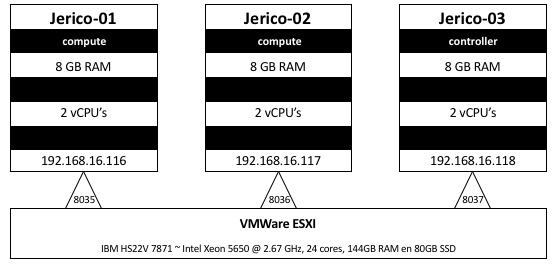
\includegraphics[scale=0.5]{Test_environment}
    }
  \end{subfigure}
  \caption{Overzicht van de testomgeving}
  \label{fig:environment}
\end{figure}

\section{DevStack}

OpenStack kan op verschillende manieren worden uitgerold zoals met Autopilot, conjure-up, alsook via DevStack. DevStack~\cite{OpenStack2017a} is een collectie van \textit{bash scripts} ontwikkeld door de community van OpenStack zelf dat volledig automatisch, mits enkele voorafgaande instellingen, OpenStack met al zijn componenten installeert en configureert. In een \textit{local.conf} bestand kunnen alle instellingen worden gewijzigd zoals de verschillende wachtwoorden, de IP-adressen, welke services actief moeten zijn, etc. Een aangemaakte stack gebruiker met \textit{sudo-}permissies kan het script uitvoeren en zo OpenStack volledig installeren op het desbetreffende systeem. \hyperref[att:installation]{Bijlage A} bevat een stap-voor-stap installatiehandleiding van OpenStack met behulp van DevStack.

Aangezien DevStack nog volop in ontwikkeling is (de huidige versie is 0.0.1\footnote{22 maart 2017}), zijn er een aantal gekende problemen. Het grootste probleem is dat OpenStack niet meer naar behoren zal werken na een heropstart van het systeem met als mogelijke oorzaak het niet opnieuw automatisch initialiseren van de daarvoor gebruikte \textit{screens} van DevStack in Ubuntu. Hierdoor worden bepaalde services niet meer gestart en is de enige mogelijkheid het opnieuw uitvoeren van het \textit{stack.sh} bestand als stack-gebruiker. Hierbij wordt alles gewist, van draaiende instanties in OpenStack tot de volledige databank die OpenStack gebruikt wat in de meeste gevallen leidt tot ongemakken. Een 'echte' oplossing voor dit probleem bestaat nog niet, maar de ontwikkeling hiervan is bezig. Een eventuele optie om dit op te lossen zijn volgende commando's:

\begin{code}
\begin{minted}[breaklines]{bash}
$ sudo su stack
$ sudo chown stack:stack `readlink /proc/self/fd/0`
$ screen -c /devstack/stack-screenrc
\end{minted}
\caption{Heropstart van DevStack na systeemherstart}
\end{code}

Dit zou de screens terug moeten koppelen aan Ubuntu en de services van OpenStack terug starten aan de hand van de services die voor de heropstart aan het draaien waren. Uitgebreide testen of dit al dan niet werkt moeten in de toekomst nog uitgevoerd worden.

Daarnaast gebeuren er bijna dagelijks \textit{commits} met verschillende oplossingen waardoor er hoogstwaarschijnlijk verschillende bugs aanwezig zijn in de gebruikte testomgeving.

\section{Nova scheduler}

OpenStack levert Nova af met een standaard \textit{filter and weighting}-scheduler die zal bepalen op welke host, ook wel \textit{hypervisor} genoemd, de nieuwe instantie geplaatst wordt. Het plaatsingsproces gebeurt in twee stappen. Eerst gaan alle beschikbare hypervisors door verschillende filters om te bepalen of de hypervisor de instantie kan hosten. Voorbeelden van standaard meegeleverde filters zijn de RamFilter, DiskFilter, AllHostFilter, en nog vele anderen. In het configuratiebestand van Nova (standaard \textit{nova.conf in /etc/nova/}) bevindt er zich een lijst met alle filters die gebruikt worden tijdens het verkiezingsproces. Zo zal de RamFilter alleen de hypervisors toelaten die voldoende RAM-geheugen ter beschikking hebben terwijl de AllHostFilter alle hypervisors zal toelaten, ongeacht deze plaats hebben voor de nieuwe instantie of niet. Vervolgens worden de toegelaten instanties gesorteerd volgens een bepaald gewicht waardoor de beste hypervisor de nieuwe instantie mag hosten. Figuur~\ref{fig:filteringWorkflow} geeft dit proces schematisch weer.

\begin{figure}
  \centering
  \captionsetup{justification=centering}
  \begin{subfigure}{\textwidth}
    \centering
    \centerline{
      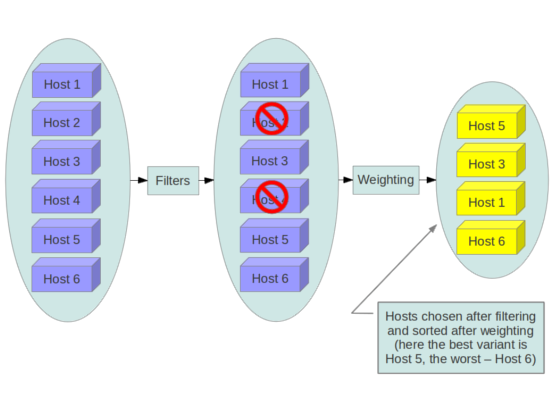
\includegraphics[scale=0.80]{filteringWorkflow1}
    }
  \end{subfigure}
  \caption{Werking van de Nova-scheduler~\cite{OpenStack2017c}}
  \label{fig:filteringWorkflow}
\end{figure}

\subsection{Round Robin scheduler}

Zoals beschreven in~\ref{sec:problem} zal er een proof-of-concept (PoC) worden uitgevoerd om de evaluatie van een resource allocatieschema aan te tonen. Hier is gekozen voor het relatief eenvoudig Round Robin schema, wat een nieuwe instantie steeds op de volgende hypervisor in de rij zal plaatsen. Een hypervisor waarbij net een nieuwe instantie is geplaatst zal zich achteraan in de rij bevinden. Concreet, de eerste instantie zal gehost worden op jerico-01, de tweede op jerico-02, de derde op jerico-03, de vierde op jerico-01 en zo verder.

Aangezien OpenStack en al zijn componenten open-source zijn, biedt het de optie om eigen nova-filters en -weighters te implementeren. Hieraan zijn wel enkele voorwaarden verbonden. Zo moet een custom-filter steeds overerven van \textit{filters} die zich in het \textit{Nova.scheduler}-pakket bevinden (ook wel de \textit{BaseHostFilter} genaamd). Bovendien moet de methode \textit{host\textunderscore passes} geïmplementeerd worden dat de waarde \textit{True} als resultaat teruggeeft indien de hypervisor geschikt is om de instantie te hosten, en \textit{False} indien de hypervisor niet geschikt is voor het hosten van de instantie.

Om het Round Robin algoritme eenvoudig in OpenStack te kunnen implementeren, is hiervoor een \textit{RoundRobinFilter} ontwikkeld. Deze laat enkel de host, die als eerste in de virtuele rij staat, toe om de nieuwe instantie te hosten. De hiervoor gebruikte code bevindt zich hieronder.

\begin{code}
\inputminted{python}{round_robin_filter.py}
\caption{RoundRobinFilter}
\end{code}


Bij iedere nieuwe aanmaak van een instantie zal elke hypervisor door deze filter passeren. Enkel de hypervisor die als eerste in de virtuele rij staat, bepaald door de \textit{counter}, zal True als resultaat van de methode teruggeven en uiteindelijk de nieuwe instantie hosten.

\subsection{Inpluggen van de Round Robin Scheduler}

Om de Round Robin scheduler te activeren in de gebruikte OpenStack omgeving moeten volgende stappen gebeuren:

\begin{enumerate}
  \item Bewaar bovenstaande code in /opt/stack/nova/nova/scheduler/filters/round\textunderscore robin\textunderscore filter.py (naam vrij te kiezen)
  \item Pas het /etc/nova/nova.conf bestand aan zodat in de [DEFAULT]-sectie de lijst van \textit{scheduler\textunderscore default\textunderscore filters} vervangen wordt door \textit{RoundRobinFilter} (naam van de klasse)
  \item Controleer ook in dit bestand of de \textit{scheduler\textunderscore driver} staat ingesteld op \textit{filter\textunderscore scheduler}
  \item Als laatste moet de Nova-scheduler worden herstart. Gebruik hiervoor het commando \textit{\$ screen -x stack} om de screens te betreden, navigeer vervolgens naar het \textit{n-sch} screen en herstart deze service door deze te stoppen (ctrl + c) en terug te starten (pijl naar boven + enter)
\end{enumerate}

Het gebruik van de screens van OpenStack staat uitgelegd in \hyperref[att:installation]{Bijlage A}.

Zoals te zien is in het \textit{nova.conf}-bestand, zijn er verschillende mogelijkheden om de scheduler van Nova te wijzigen. In dit geval is er voor een relatief eenvoudige optie gekozen om een nieuw allocatieschema te gebruiken. Meer complexere allocatieschema's zullen ook aanpassingen van de scheduler\textunderscore driver vereisen voor een correcte werking maar daar wordt niet dieper op ingegaan.

\section{FaaFo - First App Application For OpenStack}
\label{sec:faafo}

Een cloud-applicatie is optimaal indien het de mogelijkheid biedt om te schalen. FaaFo~\cite{OpenStack2017j} is een OpenStack-applicatie die fractalen, voorbeeld in Figuur~\ref{fig:fractal}, van een bepaalde grootte berekent. FaaFo is ontwikkeld door OpenStack om horizontaal uit te schalen. In dit onderzoek is FaaFo uitgerold op minimaal twee nodes. De eerste is de controller-node, die de databank en de queue beheert en de verschillende workers opdrachten kan geven om fractalen te berekenen. De twee node is bijgevolg een worker-node die een fractaal uit de queue van de controller-node zal berekenen en het resultaat zal bewaren in de databank op de controller-node.

De mogelijkheid om te schalen binnen deze applicatie komt door de goede opsplitsing van de verschillende taken in \textit{microservices} en door gebruik te maken van een queue waar de fractalen, die nog berekend moeten worden, in worden bewaard. Een optimaal scenario om te schalen zou als volgt verlopen: indien de enige worker veel CPU-kracht gebruikt binnen een bepaalde periode, dan moet er een tweede worker worden aangemaakt die de eerste worker zal helpen met al het werk. Blijken deze twee samen dan nog veel CPU-kracht te gebruiken, dan wordt een eventuele derde, vierde, ... worker aangemaakt. Indien er meer dan twee workers actief zijn en indien de queue leeg is, dan moeten de overbodige workers worden verwijderd. Dit hele proces wordt eveneens verduidelijkt in Figuur~\ref{fig:flow_chart}.

\begin{figure}
  \centering
  \captionsetup{justification=centering}
  \begin{subfigure}{\textwidth}
    \centering
    \centerline{
      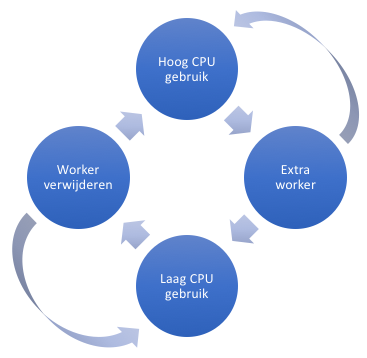
\includegraphics[scale=0.50]{flow_chart}
    }
  \end{subfigure}
  \caption{FaaFo: het schaalscenario}
  \label{fig:flow_chart}
\end{figure}

Het scenario is sterk gerelateerd aan de werkelijke gang van zaken binnen cloud computing. Zoals beschreven in Sectie~\ref{sec:what_is_cloud_computing} en in Sectie~\ref{sec:rmcloud} moet een cloud-gebruiker enerzijds schalen zodat de SLA tegenover hun eindgebruikers wordt voldaan en anderzijds de kosten voor het gebruik van de resources van de cloud provider worden geminimaliseerd. Doordat de applicatie bij hoge werklast horizontaal zal uitschalen, kan de SLA tegenover de eindgebruiker worden voldaan (de fractaal zal snel berekend worden) en bij te weinig werk zal de applicatie horizontaal krimpen zodat er minder resources gebruikt worden en er minder kosten zijn aan de cloud-provider.

\subsection{Schalen binnen OpenStack}

\begin{figure}
  \centering
  \captionsetup{justification=centering}
  \begin{subfigure}{\textwidth}
    \centering
    \centerline{
      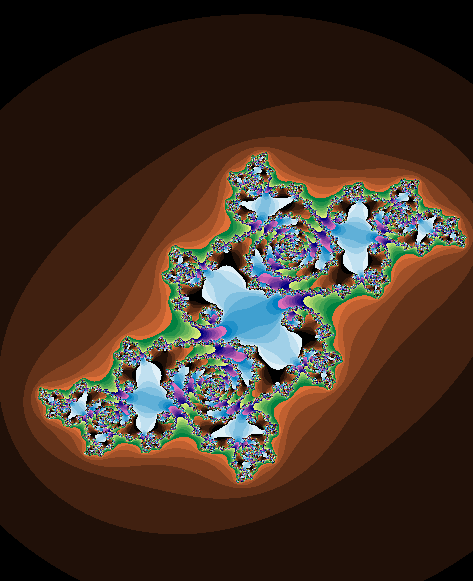
\includegraphics[scale=0.30]{fractal-example}
    }
  \end{subfigure}
  \caption{Voorbeeld van een fractaal}
  \label{fig:fractal}
\end{figure}

Zoals vermeld in Sectie~\ref{sec:Openstack} bevat OpenStack verschillende  componenten, waaronder ook een aantal die het mogelijk maken om applicaties automatisch te schalen. De combinatie van de Orchestration-~\cite{OpenStack2017g} en de Telemetry-services~\cite{OpenStack2017h} zorgt ervoor dat automatisch schalen mogelijk wordt. \textit{Heat} biedt de mogelijkheid om meer of minder instanties aan te maken afhankelijk van de vraag. \textit{Ceilometer} en \textit{Aodh} zorgen voor de monitoring van bepaalde instanties om zo te bepalen of het wel nuttig is om te schalen. Aan de hand van alarmen zullen deze twee componenten Heat op de hoogte brengen van de situatie van de verschillende instanties, waarop Heat op zijn beurt zal reageren door het aanmaken van een nieuwe instantie, een instantie te verwijderen of het alarm te negeren.

Het gehele gebeuren van alarmen, schalen, etc. gebeurt in OpenStack met een \textit{stack}~\cite{OpenStack2017i}. Een stack is een verzameling van OpenStack resources zoals instanties, IP-adressen, volumes, gebruikers, etc die gecreëerd worden met een \textit{template}. Zulke template, geschreven in OpenStack Heat Orchestration Template (HOT)~\cite{OpenStack2017f} formaat of Amazon Web Services (AWS) formaat, is een beschrijving van de gebruikte instanties, gebruikers, images, alarmen, etc.

\subsection{FaaFo met OpenStack SDK - Libcloud}

Een eerste mogelijkheid om FaaFo te configureren en installeren is met behulp van LibCloud~\cite{Libcloud}, een Python-bibliotheek voor interactie met verschillende cloud service providers. Deze werd reeds kort aangehaald in Sectie~\ref{sec:related_work}. De code is grotendeels gebaseerd op een handleiding van OpenStack zelf~\cite{OpenStack2017k}, mits enkele kleine aanpassingen.

De code bestaat uit verschillende stappen en is beschikbaar via GitHub.\footnote{\url{https://github.ugent.be/jfmoeyer/EvaluationRASOpenStack/blob/master/application/firstapplication.py}} Na het initialiseren van de cloud provider en indien er een connectie is gemaakt kan de eerste stap beginnen. Deze print alle images alsook alle flavors uit. Ook zal er een specifieke image en flavor geselecteerd worden voor verder gebruik. De tweede stap gaat een instantie maken, alle instanties printen en dan deze instantie terug verwijderen. In de derde stap gebeurt een configuratie die helpt om de werking van OpenStack zelf te begrijpen. Hierin wordt er eerst een sleutelpaar aangemaakt met de naam \textit{demokey} indien deze nog niet bestaat. Dit sleutelpaar is nodig om een SSH-verbinding met de instantie mogelijk te maken. Enkel de gebruikers die dezelfde sleutel bevatten als diegene waarmee de instantie is geïnitialiseerd, zullen een SSH-verbinding kunnen maken. Naast een sleutelpaar worden er ook enkele \textit{security groups} aangemaakt die dienst doen als een soort \textit{firewall}. Standaard blokkeren de instanties alle inkomende en uitgaande verbindingen\footnote{In firewall-termen: de default policy is block/discard} waardoor er nood is aan het toelaten van enkele connecties zoals bijvoorbeeld een SSH-connectie (poort 22) vanaf de OpenStack-controller. In de vierde stap wordt met de vorige instellingen en configuratie een instantie gestart die de FaaFo-applicatie zal uitvoeren (all-in-one). De volgende stappen zijn gelijkaardig zodat de FaaFo-applicatie wordt opgesplitst in een FaaFo-API voor de API-services, een FaaFo-controller voor de arbitrage en een FaaFo-worker voor de eigenlijke berekeningen. Hier wordt gebruik gemaakt van een \textit{floating ip}, nodig om een externe connectie, bijvoorbeeld een SSH-verbinding, te maken met de instantie. De standaard toegewezen IP-adressen zijn enkel bruikbaar voor de communicatie tussen de instanties zelf.

De FaaFo-applicatie heeft via LibCloud niet de mogelijkheid om te schalen waardoor het niet bruikbaar is voor de Proof-of-Concept. Toch is dit hele proces geen verloren zaak geweest doordat de werking van OpenStack duidelijker is geworden en de derde stap nog gebruikt wordt voor de configuratie van het sleutelpaar.

\subsection{FaaFo \& OpenStack-Orchestration: een schaalbare cloudapplicatie}
\label{sec:faafo_template}

Om een schaalbare FaaFo-applicatie uit te rollen moet er gebruik gemaakt worden van een HOT-template of een AWS-template. In deze thesis is gekozen voor het HOT-formaat omdat het onderdeel is van OpenStack en omdat er voldoende informatie beschikbaar is. In onderstaande paragrafen bevinden zich delen van de code met de nodige informatie. De volledige code is te vinden op Github.\footnote{\url{https://github.ugent.be/jfmoeyer/EvaluationRASOpenStack/blob/master/application/autoscaling_workers.yaml}}

De volledige template bevat twee grote delen, namelijk de parameters en de resources. De parameters, weergegeven in Listing~\ref{lst:faafo_param}, beschrijven de variabelen die worden meegegeven door de gebruiker. Zo zal de \textit{key\textunderscore name} bepalen welke SSH-sleutel gebruikt wordt voor de toegang tot de instanties zodat niet iedereen toegang heeft. De \textit{flavor} beschrijft welke hardware de instantie ter beschikking heeft en de \textit{image\textunderscore id} beschrijft het besturingssysteem voor de instantie. De laatste drie parameters beschrijven de periode voor het monitoren en de gebruikte scripts zodat de nieuwe instanties bepaalde code automatisch kunnen uitvoeren. Deze 3 parameters zijn optioneel aangezien er een \textit{default}-waarde aan is toegekend.

\begin{code}
\begin{minted}[frame=bottomline, fontsize=\footnotesize]{yaml}
heat_template_version: 2014-10-16
description: |
A template that starts auto-scaling workers for the faafo application

parameters:
  key_name:
    type: string
    description: Name of the keypair to enable ssh
    default: id_rsa
    constraints:
      - custom_constraint: nova.keypair
      description: Must already exist on the cloud

  flavor:
    type: string
    description: The flavor that the application uses
    constraints:
      - custom_constraint: nova.flavor
      description: Must be a valid flavor provided by the cloud provider.

  image_id:
    type: string
    description: The ID fo the image for the creation of the instances.
    constraints:
      - custom_constraint: glance.image
      description: Must be a valid image on your cloud

  period:
    type: number
    description: The period to use to calculate the ceilometer statistics (in seconds)
    default: 60

  worker_source:
    type: string
    description: The location of the installation script for the workers
    default: https://raw.githubusercontent.com/moeyerke/nodejs-agent/master/userdata_workers.sh

  controller_source:
    type: string
    description: The location of the installation script for the controller
    default: https://raw.githubusercontent.com/moeyerke/nodejs-agent/master/userdata_controller.sh
\end{minted}
\caption{FaaFo-template: de parameters}
\label{lst:faafo_param}
\end{code}

De resources-sectie bevat de eigenlijke essentie van de template. Deze bestaat uit de \textit{security groups}, welke vergelijkbaar zijn met een firewall, servers, \textit{scaling groups} en alarmen. Als eerste worden twee \textit{security groups} aangemaakt, één voor de worker-instanties en één voor de controller-instantie, beiden weergegeven in Listing~\ref{lst:faafo_sec}. De \textit{security group} van de worker laat enkel een SSH-connectie (poort 22) toe vanuit jerico-03, de controller-node van OpenStack. De security group van de FaaFo controller-instantie is uitgebreider. Hier wordt naast het toelaten van een SSH-verbinding vanuit jerico-03 ook een HTTP-verbinding toegestaan en toegang voor de worker-instanties tot poort 5672 (gebruikt door de queue).

\begin{code}
\begin{minted}[breaklines]{yaml}
resources:
  worker:
    type: OS::Neutron::SecurityGroup
    properties:
      description: "Enables ssh to worker node"
      rules: [
        {remote_ip_prefix: 0.0.0.0/0,
        protocol: tcp,
        port_range_min: 22,
        port_range_max: 22},]

  controller:
    type: OS::Neutron::SecurityGroup
    properties:
      description: "For services that run on a control node"
      rules: [
        {remote_ip_prefix: 0.0.0.0/0,
        protocol: tcp,
        port_range_min: 5672,
        port_range_max: 5672,
        remote_mode: remote_group_id,
        remote_group_id: { get_resource: worker } },
        {remote_ip_prefix: 0.0.0.0/0,
        protocol: tcp,
        port_range_min: 80,
        port_range_max: 80},
        {remote_ip_prefix: 0.0.0.0/0,
        protocol: tcp,
        port_range_min: 22,
        port_range_max: 22},
      ]
\end{minted}
\caption{FaaFo-template: de security groups}
\label{lst:faafo_sec}
\end{code}

Vervolgens wordt er een Nova-server, de FaaFo controller-instantie aangemaakt met de meegegeven \textit{key\textunderscore name}, \textit{flavor} en \textit{image}. Het aanmaken van de controller-instantie bevindt zich in Listing~\ref{lst:faafo_controller}. De \textit{user\textunderscore data} beschrijft het commando dat wordt uitgevoerd na het opstarten van de instantie. In \hyperref[att:scripts]{Bijlage C} worden de scripts toegelicht.

\begin{code}
\begin{minted}[breaklines]{yaml}
  controller_instance:
    type: OS::Nova::Server
    properties:
      key_name: { get_param: key_name }
      image: { get_param: image_id }
      flavor: { get_param: flavor }
      name: app-controller
      security_groups:
        - {get_resource: controller}
      user_data_format: RAW
      user_data:
        str_replace:
          template: |
            #!/usr/bin/env bash
            curl -L -s controller_source | bash
          params:
            controller_source: { get_param: controller_source }
\end{minted}
\caption{FaaFo-template: de controller-instantie}
\label{lst:faafo_controller}
\end{code}

Naast de FaaFo controller-instantie moeten er ook worker-instanties worden aangemaakt, weergegeven in Listing~\ref{lst:faafo_scaling}. Omdat deze het meeste werk zullen verrichten (en dus veel CPU-resources zullen verbuiken), moeten deze kunnen horizontaal schalen. De \textit{AutoScalingGroup} beschrijft de worker-instantie met dezelfde parameters als de controller-instantie (met uitzondering van de \textit{security group} en de \textit{user\textunderscore data}-parameter). Belangrijke parameters bij de \textit{AutoScalingGroup} zijn de onderste drie, namelijk \textit{min\textunderscore size, desired\textunderscore capacity en max\textunderscore size}, die bepalen hoeveel worker-instanties actief kunnen zijn, en aan hoeveel actieve instanties de voorkeur gegeven wordt.


\begin{code}
\begin{minted}[breaklines]{yaml}
  worker_auto_scaling_group:
    #The worker instances are managed by this auto_scaling group
    type: OS::Heat::AutoScalingGroup
    properties:
      resource:
        type: OS::Nova::Server
        properties:
          key_name: { get_param: key_name }
          image: { get_param: image_id }
          flavor: { get_param: flavor }
          name: worker
          security_groups:
            - {get_resource: worker}
          user_data_format: RAW
          user_data:
            str_replace:
              template: |
                #!/usr/bin/env bash
                curl -L -s worker_source | bash -s -- controller_ip1 controller_ip2
              params:
                controller_ip1: { get_attr: [controller_instance, networks, private, 0] }
                controller_ip2: { get_attr: [controller_instance, networks, private, 1] }
                worker_source: { get_param: worker_source }
      min_size: 1
      desired_capacity: 1
      max_size: 7
\end{minted}
\caption{FaaFo-template: de AutoScalinGroup}
\label{lst:faafo_scaling}
\end{code}

Nadien worden er in Listing~\ref{lst:faafo_scaling_policies} twee \textit{ScalingPolicies} gedefinieerd, de ene om omhoog te schalen, de andere om omlaag te schalen. Hierbij wordt telkens vermeld welke instanties er moeten bijgemaakt of verwijderd worden en met hoeveel tegelijkertijd. In deze template gaat het dus over de worker-instanties die telkens met 1 instantie worden verhoogd of verlaagd.

\begin{code}
\begin{minted}[breaklines]{yaml}
  scale_up_policy:
    type: OS::Heat::ScalingPolicy
    properties:
      adjustment_type: change_in_capacity
      auto_scaling_group_id: {get_resource: worker_auto_scaling_group}
      cooldown: { get_param: period }
      scaling_adjustment: 1

  scale_down_policy:
    type: OS::Heat::ScalingPolicy
    properties:
      adjustment_type: change_in_capacity
      auto_scaling_group_id: {get_resource: worker_auto_scaling_group}
      cooldown: { get_param: period }
      scaling_adjustment: '-1'
\end{minted}
\caption{FaaFo-template: de ScalingPolicies}
\label{lst:faafo_scaling_policies}
\end{code}

Als laatste worden er twee alarmen geconfigureerd in Listing~\ref{lst:faafo_alarms}, één indien er zeer veel activiteit op de worker-instanties is en één indien er weinig activiteit is. De alarmen gaan in dit geval het gebruik van de CPU monitoren gedurende een bepaalde periode (standaard 60s) en indien de \textit{treshold} overschreden wordt, zal het alarm een \textit{ScalePolicy} triggeren die op zijn beurt een extra worker-instantie zal toevoegen of verwijderen.

\begin{code}
\begin{minted}[breaklines]{yaml}
  cpu_alarm_high:
    type: OS::Aodh::Alarm
    properties:
      description: Scale-up if the average CPU > 90 % for period of seconds
      meter_name: cpu_util
      statistic: avg
      period: { get_param: period }
      evaluation_periods: 1
      threshold: 90
      alarm_actions:
        - {get_attr: [scale_up_policy, alarm_url]}
      comparison_operator: gt

  cpu_alarm_low:
    type: OS::Aodh::Alarm
    properties:
      description: Scale-down if the average CPU < 15 % for period of seconds
      meter_name: cpu_util
      statistic: avg
      period: { get_param: period }
      evaluation_periods: 1
      threshold: 15
      alarm_actions:
        - {get_attr: [scale_down_policy, alarm_url]}
      comparison_operator: lt
\end{minted}
\caption{FaaFo-template: de alarmen}
\label{lst:faafo_alarms}
\end{code}

\subsection{Problemen met de applicatie}
\label{sec:faafoproblems}

Desondanks dat de FaaFo-applicatie ontwikkeld is door OpenStack waren er nog een hele reeks problemen die opgelost moesten worden vooraleer het hele gebeuren correct werkte. Deze problemen worden hier kort toegelicht samen met de eventuele oplossing.

Het grootste probleem met de FaaFo-applicatie had te maken met de manier waarop deze wordt geïmplementeerd in bovenstaande Listings en de werking van Ceilometer/Aodh. Door in de configuratie van de alarmen geen \textit{query} of metadata mee te geven baseert Ceilometer zich op metingen van alle actieve instanties. Dit heeft als gevolg dat de applicatie op sommige ogenblikken een worker zal verwijderen omdat het \textit{cpu\textunderscore alarm\textunderscore low} wordt getriggerd door de lezing van een instantie die totaal niets met de applicatie heeft te maken. OpenStack heeft hiervoor een oplossing beschreven in~\cite{OpenStack2017j}. Bij de alarmen wordt een \textit{matching\textunderscore metadata} geconfigureerd en bij de \textit{AutoScalingGroup} wordt er metadata meegegeven. Deze configuratie moet ervoor zorgen dat Ceilometer enkel de instanties monitort met dezelfde metadata, maar na het uittesten hiervan blijkt dit niet te werken door verschillende updates van OpenStack, Ceilometer en Aodh. Ceilometer houdt in dit geval nu over niets meer toezicht en bijgevolg wordt er ook niet geschaald. Een werkende, maar niet per se een betere, oplossing is gebaseerd op voorgaande configuratie maar configureert in de alarmen nu een \textit{query}, die controleert of de naam van de instantie gelijk is aan 'worker'. Bij de \textit{AutoScalingGroup} wordt als metadata dan de naam worker meegegeven zodat enkel deze instanties invloed zullen hebben op het schalen.
In onderstaande Listing bevindt zich de aanvulling op bovenstaande Listings met de werkende metadata- en query-instellingen:

\begin{code}
\begin{minted}[breaklines]{yaml}
...
resources:
  worker_auto_scaling_group:
    ...
    properties:
      resource:
        ...
        properties:
          ...
          metadata: { "display_name": "worker" }
  ...
  cpu_alarm_high:
    ...
    properties:
      ...
      query:
        - field: metdata.display_name
           op: eq
           value: 'worker'

  cpu_alarm_low:
    ...
    properties:
      ...
      query:
        - field: metadata.display_name
           op: eq
           value: 'worker'
  ...
\end{minted}
\caption{FaaFo template met metadata}
\label{lst:faafo_add}
\end{code}

Een tweede probleem had te maken met de beveiliging van RabbitMQ, de \textit{queue} die gebruikt wordt voor de communicatie tussen de FaaFo-controller en de FaaFo-workers. Standaard gebruikt FaaFo de login-gegevens \textit{guest:guest} om te communiceren met de \textit{queue} op de FaaFo-controller. Door een eerdere update van RabbitMQ (sinds versie 3.3.0)\footnote{\url{http://www.rabbitmq.com/release-notes/README-3.3.0.txt}} zijn deze gegevens enkel bruikbaar vanaf de lokale host, en niet meer vanaf een externe host. Om dit probleem op te lossen wordt er bij de FaaFo-controller in de \textit{user\textunderscore data} een nieuwe RabbitMQ-gebruiker aangemaakt die alle permissies krijgt vanop eender welke host. Hierdoor is communicatie wel mogelijk tussen de FaaFo-controller en de FaaFo-workers. De gebruikte code bevindt zich in \hyperref[att:scripts]{Bijlage C}.

Na het oplossen van bovenstaande twee problemen werkt de applicatie grotendeels. Er is nog één probleem dat meer tijd en kennis vereiste om op te lossen en waarmee rekening moet gehouden worden tijdens de evaluaties van de allocatieschema's. Het berekenen van een fractaal kan een bepaalde tijd in beslag nemen met een hoog CPU-verbruik. Indien er meerdere worker-instanties actief zijn waarvan er één nog geen fractaal aan het bereken is en Ceilometer net die instantie monitort, kan het zijn dat er een worker-instantie wordt verwijderd omdat het alarm van laag CPU-gebruik afgaat. Is de verwijderde worker bezig met het berekenen van een fractaal, dan verdwijnt dit fractaal mee met de instantie waardoor het nooit volledig berekend zal worden. In deze context is dit probleem niet erg omdat er vooral wordt gekeken naar waar de instanties geplaatst worden, maar indien een applicatie cruciale berekeningen moet uitvoeren, mogen deze berekeningen natuurlijk niet verdwijnen.

Een mogelijke oplossing voor dit laatste probleem is de FaaFo-applicatie zo ontwikkelen dat een instantie pas verwijderd kan worden indien alle berekeningen op die specifieke instantie voltooid en doorgestuurd zijn naar de FaaFo-controller.
%\chapter{Monitoring}
\label{chap:monitoring}

Nu de gehele testomgeving geconfigureerd en werkende is, dient het hele gebeuren gemonitord worden. Dit is nodig om verschillende gegevens te verzamelen zodat er nadien kan worden overgegaan tot het evalueren van het allocatieschema in de proof-of-concept. In dit hoofdstuk wordt eerst dieper ingegaan op één specifieke tool, namelijk Rally~\cite{OpenStack2017b}, dat de deployment van OpenStack kan verifiëren. Vervolgens zal er een overzicht gegeven worden van de verschillende monitortechnieken waarna er ten slotte dieper wordt ingegaan op de gebruikte monitortechniek.

\section{Rally: evalueren schaalbaarheid OpenStack}
\label{sec:rally}

Rally~\cite{OpenStack2017b} is een benchmarking tool dat een OpenStack deployment kan automatiseren, de uitgerolde cloud kan verifiëren, benchmark testen kan uitvoeren en de cloud profileren. Het biedt daardoor een antwoord op de vraag hoe OpenStack werkt op grote schaal. Rally wordt gebruikt in drie high-level use cases die zeer interessant zijn om de deployment van OpenStack te evalueren. Een eerste use case is de mogelijkheid om een OpenStack omgeving te deployen, te testen en afhankelijk van de testresultaten OpenStack opnieuw te deployen met een andere configuratie tot de testen succesvol zijn. De tweede use case is bedoeld voor DevOps waarbij een bestaande cloud getest wordt met een simulatie van echte gebruikerswerklast waarna de resultaten worden weergegeven in allerhande grafieken. Een interessante eigenschap hierbij is dat SLA's gedefinieerd kunnen worden zodat hiermee rekening wordt gehouden tijdens het uitvoeren van de testen. De laatste use case is Rally CI/CD\footnote{\textit{Continuous Integration} en\textit{ Continuous Deployment}}, waarbij OpenStack wordt uitgerold op specifieke hardware met de laatste versie van een eigen geschreven tool. Hierop worden dan testen uitgevoerd die nadien gedeeld worden met de OpenStack community om zo OpenStack te verbeteren in de toekomst.

Rally maakt gebruik van 2 types invoerbestanden, namelijk een standaard JSON-bestand, of een YAML-bestand, een template-syntax gebaseerd op Jinja2\footnote{Een template engine geschreven in pure Python}. Elk invoerbestand bevat dan één of meerdere scenario's, al dan niet met meerdere configuraties per scenario. De configuratie van een scenario bevat steeds een lijst met argumenten (args) zoals de te gebruiken flavor, image, parameters, etc., de context die de gesimuleerde gebruikers representeert en een runner die bepaalt hoe de test wordt uitgevoerd. Optioneel kan er een nog een SLA, zoals bijvoorbeeld maximum aantal seconden per iteratie en de \textit{failure rate}, toegevoegd worden dat de eigenlijke succescriteria omschrijft.

Een voorbeeld om Rally beter te leren begrijpen maakt gebruik van een \textit{sample} invoerbestand en toont het verschil tussen een \textit{all-in-one} OpenStack deployment en een multi-node OpenStack deployment. Het invoerbestand ziet eruit als volgt:

\begin{code}
\begin{minted}[breaklines, fontsize=\footnotesize]{json}
{ % set flavor_name = flavor_name or "m1.tiny" %}
{  "NovaServers.boot_and_delete_server": [{
    "args": {
    "flavor": {
      "name": "{{flavor_name}}"
    },
    "image": {
      "name": "^cirros.*-disk$"
    },
    "force_delete": false
  },
  "runner": {
    "type": "constant",
    "times": 10,
    "concurrency": 2
  },
  "context": {
    "users": {
      "tenants": 3,
      "users_per_tenant": 2
      }}}, {
    "args": {
      "flavor": {
        "name": "{{flavor_name}}"
        },
      "image": {
        "name": "^cirros.*-disk$"
        },
      "auto_assign_nic": true
    },
    "runner": {
      "type": "constant",
      "times": 10,
      "concurrency": 2
    },
    "context": {
      "users": {
        "tenants": 3,
        "users_per_tenant": 2
      },
      "network": {
        "start_cidr": "10.2.0.0/24",
        "networks_per_tenant": 2
      }}}]}
\end{minted}
\caption{Rally test}
\end{code}

Dit invoerbestand stelt een scenario, NovaServers.boot\textunderscore and\textunderscore delete\textunderscore server, voor met twee configuraties. De eerste configuratie maakt gebruik van de flavor m1.tiny tenzij er een andere wordt meegegeven op de commandolijn, de standaard meegeleverde cirros image en de force\textunderscore delete option ingesteld op false. De runner-instelling bepaalt dat het proces 10 keer herhaald wordt waarbij er twee iteraties tegelijkertijd kunnen gebeuren (concurrency) en de context stelt de 6 gebruikers voor, verdeeld over 3 tenants. De tweede configuratie is grotendeels dezelfde als de eerste en bovendien wordt er een extra network-optie meegegeven.

Met bovenstaand invoerbestand kan de test worden uitgevoerd, eerst op een all-in-one omgeving met 1 node, vervolgens op de testomgeving zoals beschreven in Hoofdstuk~\ref{sec:environment}. De test uitvoeren gebeurt via volgend commando:

\begin{code}
\begin{minted}[breaklines]{bash}
$ rally task start `/opt/stack/rally/samples/tasks/scenarios/nova/
boot-and-delete.json`
\end{minted}
\end{code}

Na het uitvoeren van de test zijn de resultaten beschikbaar voor exporteren. Via volgend commando worden de resultaten geëxporteerd in een HTML-bestand:

\begin{code}
\begin{minted}[breaklines]{bash}
$ rally task report --out=report1.html
\end{minted}
\end{code}

Na het uitvoeren van de testen op beide omgevingen zijn er twee rapporten beschikbaar, één voor elke omgeving. De belangrijkste gegevens worden weergegeven in Figuur~\ref{fig:rally-test1} en Figuur~\ref{fig:rally-test2} en hierna besproken. De bovenste grafieken stellen de resultaten van de eerste configuratie voor, de onderste grafieken stellen de resultaten van de twee configuratie voor.

\begin{figure}
  \centering
  \captionsetup{justification=centering}
  \begin{subfigure}{\textwidth}
    \centering
    \centerline{
      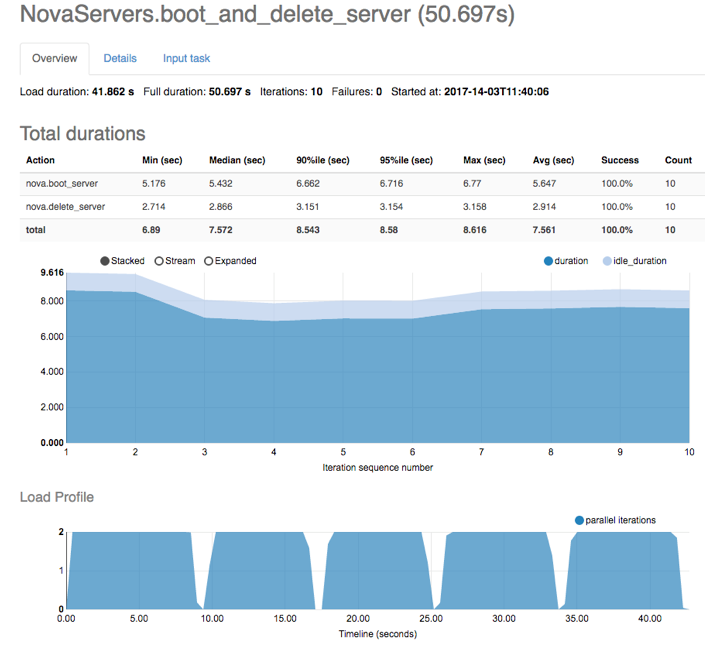
\includegraphics[scale=0.70]{Dia1}
    }
  \end{subfigure}
  \caption{Resultaat Rally-test: All-in-One Node}
  \label{fig:rally-test1}
\end{figure}

\begin{figure}
  \centering
  \captionsetup{justification=centering}
  \begin{subfigure}{\textwidth}
    \centering
    \centerline{
      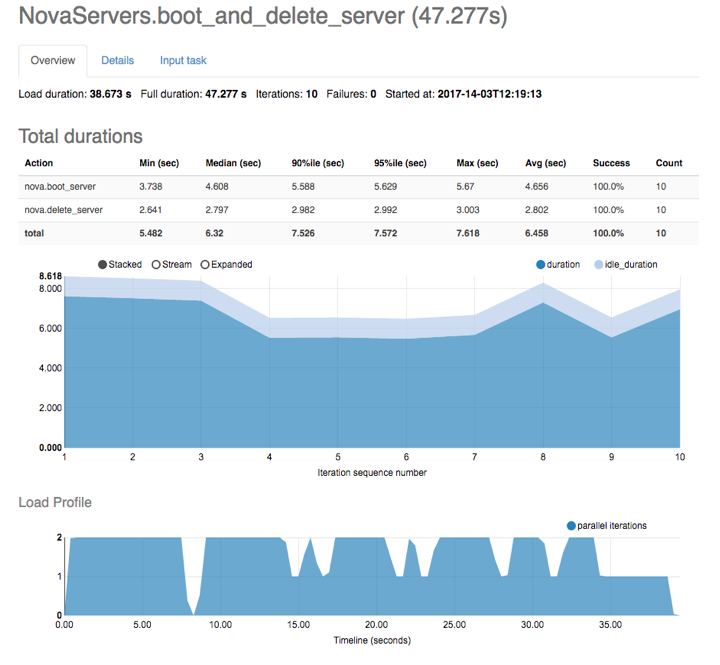
\includegraphics[scale=0.70]{Dia2}
    }
  \end{subfigure}
  \caption{Resultaat Rally-test: Testomgeving}
  \label{fig:rally-test2}
\end{figure}

Zoals te zien bovenaan in Figuur~\ref{fig:rally-test1} en Figuur~\ref{fig:rally-test2} is er een duidelijk verschil in de \textit{Load Profile} grafieken tussen beide opstellingen. Deze stellen het aantal parallelle iteraties voor in functie van de tijd en hieruit is duidelijk dat de testomgeving parallellisme beter ondersteund. Ook de tijd om een instantie te starten en te verwijderen is 12\% tot 20\% beter in de testomgeving dan in de all-in-one omgeving.
In de onderste grafieken is het meteen duidelijk dat de all-in-one opstelling faalt bij de laatste twee iteraties in tegenstelling tot de testomgeving. De tijd om een instantie te starten en te verwijderen is 16\% tot 27\% beter in de testomgeving dan in de all-in-one omgeving en het Load Profile is constanter in de testomgeving wat zorgt voor een betere betrouwbaarheid.

De testen uitgevoerd door Rally zijn nuttig om een nieuwe Nova-scheduler te evalueren op high-level niveau. Het ontwikkelen van een eigen test op een aangepaste Nova-scheduler biedt de mogelijkheid om deze nieuwe scheduler te testen met een vari"erende werklast waarbij de resultaten nadien eenvoudig worden omgezet in grafieken. Een belangrijk aspect is dat hiermee bekeken wordt of de nieuwe scheduler niet faalt om nieuwe instanties te creëren bij een stijgende werklast.

\section{Mogelijkheden om te monitoren}

Deze sectie geeft een overzicht weer van de verschillende mogelijkheden om een OpenStack-cloud te monitoren en data te verzamelen. Elke mogelijkheid zal tevens ook kort worden toegelicht met een eventueel voorbeeld.

\subsection{Nodejs-agent}
\label{sec:nodejs-agent}

Het monitoren van de drie hypervisors zal gebeuren met behulp van een zelf ontwikkelde Node.js-agent. Deze applicatie is een Node.js-applicatie die zal draaien op elk van de hypervisors. Met behulp van \textit{Express}, een \textit{npm package}, wordt er een node-server geïnitialseerd en gestart die vervolgens zal luisteren naar aanvragen op een vooraf ingestelde poort. Op dit ogenblik zijn volgende aanvragen geïmplementeerd:

\begin{itemize}
  \item \textit{/ping}: verwacht geen query, en geeft een 1 terug als resultaat (\textit{text/plain})
  \item \textit{/mongodb}: verwacht geen query, en geeft een JSON-string terug met het huidig resource-verbruik (\textit{application/json})
  \item \textit{/periodstats}: verwacht een query met 2 parameters, start en stop, waarbij beiden een tijdstip omschrijven met als vorm yyyy-dd-mmThh:mm:ss.xxxZ en geeft een JSON-string terug met het resource-verbruik tussen de twee meegegeven tijdstippen (\textit{application/json})
  \item \textit{/ceilometerstats}: verwacht een query met 2 parameters, start en stop, waarbij beiden een tijdstip omschrijven met als vorm yyyy-dd-mmThh:mm:ss.xxxZ en geeft een JSON-string terug met de metingen van Ceilometer tussen de twee meegegeven tijdstippen (\textit{application/json})
  \item \textit{/timestats}: verwacht een query met 2 parameters, start en stop, waarbij beiden een tijdstip omschrijven met als vorm yyyy-dd-mmThh:mm:ss.xxxZ en geeft een JSON-string terug met het resource-verbruik tussen de twee meegegeven tijdstippen alsook de metingen van ceilometer, beiden geordend volgens tijdstip (\textit{application/json})
\end{itemize}

De ping-aanvraag geeft eenvoudig weer of de agent op de hypervisor bereikbaar en geactiveerd is door een 1 terug te sturen naar de aanvrager. De mongodb aanvraag is belangrijk voor de correcte werking van de andere aanvragen. Indien de agent zo een aanvraag krijgt zal hij met behulp van het node-package \textit{os-utils} het CPU-verbruik en de hoeveelheid vrij geheugen bepalen. Vervolgens zal de agent met behulp van het node-package \textit{mysql} een connectie maken met de MySQL-databank op de OpenStack-controller, namelijk jerico-03, om de hoeveelheid actieve instanties op te vragen die op de hypervisor gehost zijn. Al deze resultaten samen met het huidige tijdstip worden dan bewaard in een mongoDB-databank welke actief is op jerico-01. Deze resultaten worden ook teruggezonden naar de aanvrager in JSON-formaat en kunnen nadien ook opgevraagd worden via de andere aanvragen (met uitzondering van de ping aanvraag).

Indien een aanvraag wordt gestuurd naar periodstats samen met twee parameters, een start- en eindtijdstip, zal de agent alle data van alle hypervisors tussen deze twee tijdstippen opvragen van de mongoDB op jerico-01. Een aanvraag naar ceilometerstats is gelijkaardig, enkel zal hier een aanvraag worden gestuurd naar de MongoDB op jerico-03 om zo alle statistieken die Ceilometer gemeten heeft binnen de meegegeven periode terug te geven aan de aanvrager. De timestats-aanvraag is een combinatie van de laatste twee, mits enkele aanpassingen. Zo wordt de data van ceilometer opnieuw opgevraagd van de MongoDB op jerico-03 en worden ook de instanties van de MySQL-databank op jerico-03 opgevraagd, beiden met het bijhorende tijdstip. Een combinatie van deze resultaten wordt nadien bezorgd aan de aanvrager.

\subsection{Grafana}

Grafana~\cite{Labs} is een van de meest bekende open-source software voor tijdsreeksanalyse. Het biedt een krachtige en elegante manier aan voor het creëren, ontdekken en delen van dashboards en data met een team of de hele wereld. Dankzij verschillende plugins is het mogelijk om variërende panelen, die onder andere grafieken bevatten, te configureren en te analyseren.

Ook een OpenStack-cloud kan met Grafana gemonitord en geanalyseerd worden indien aan bepaalde voorwaarden voldaan is. Zo moet OpenStack gebruikmaken van de Gnocchi-database waar Ceilometer zijn statistieken zal bewaren. Gnocchi~\cite{OpenStack2017d} is een projectnaam voor een TDBaaS (Time Series Database as a Service) project dat moet samenwerken met OpenStack Ceilometer. Het voordeel van deze benadering is dat vele metrieken, van de temperatuur tot het CPU-gebruik, worden bewaard per tijdstip en zo eenvoudig kunnen worden opgevraagd. Grafana kan dan met behulp van de Gnocchi-plugin\footnote{\url{https://grafana.com/plugins/sileht-gnocchi-datasource}} en de nodige configuratie een volledige OpenStack-cloud monitoren met een mogelijk resultaat zoals in Figuur~\ref{fig:grafana}.

\begin{figure}
  \centering
  \captionsetup{justification=centering}
  \begin{subfigure}{\textwidth}
    \centering
    \centerline{
      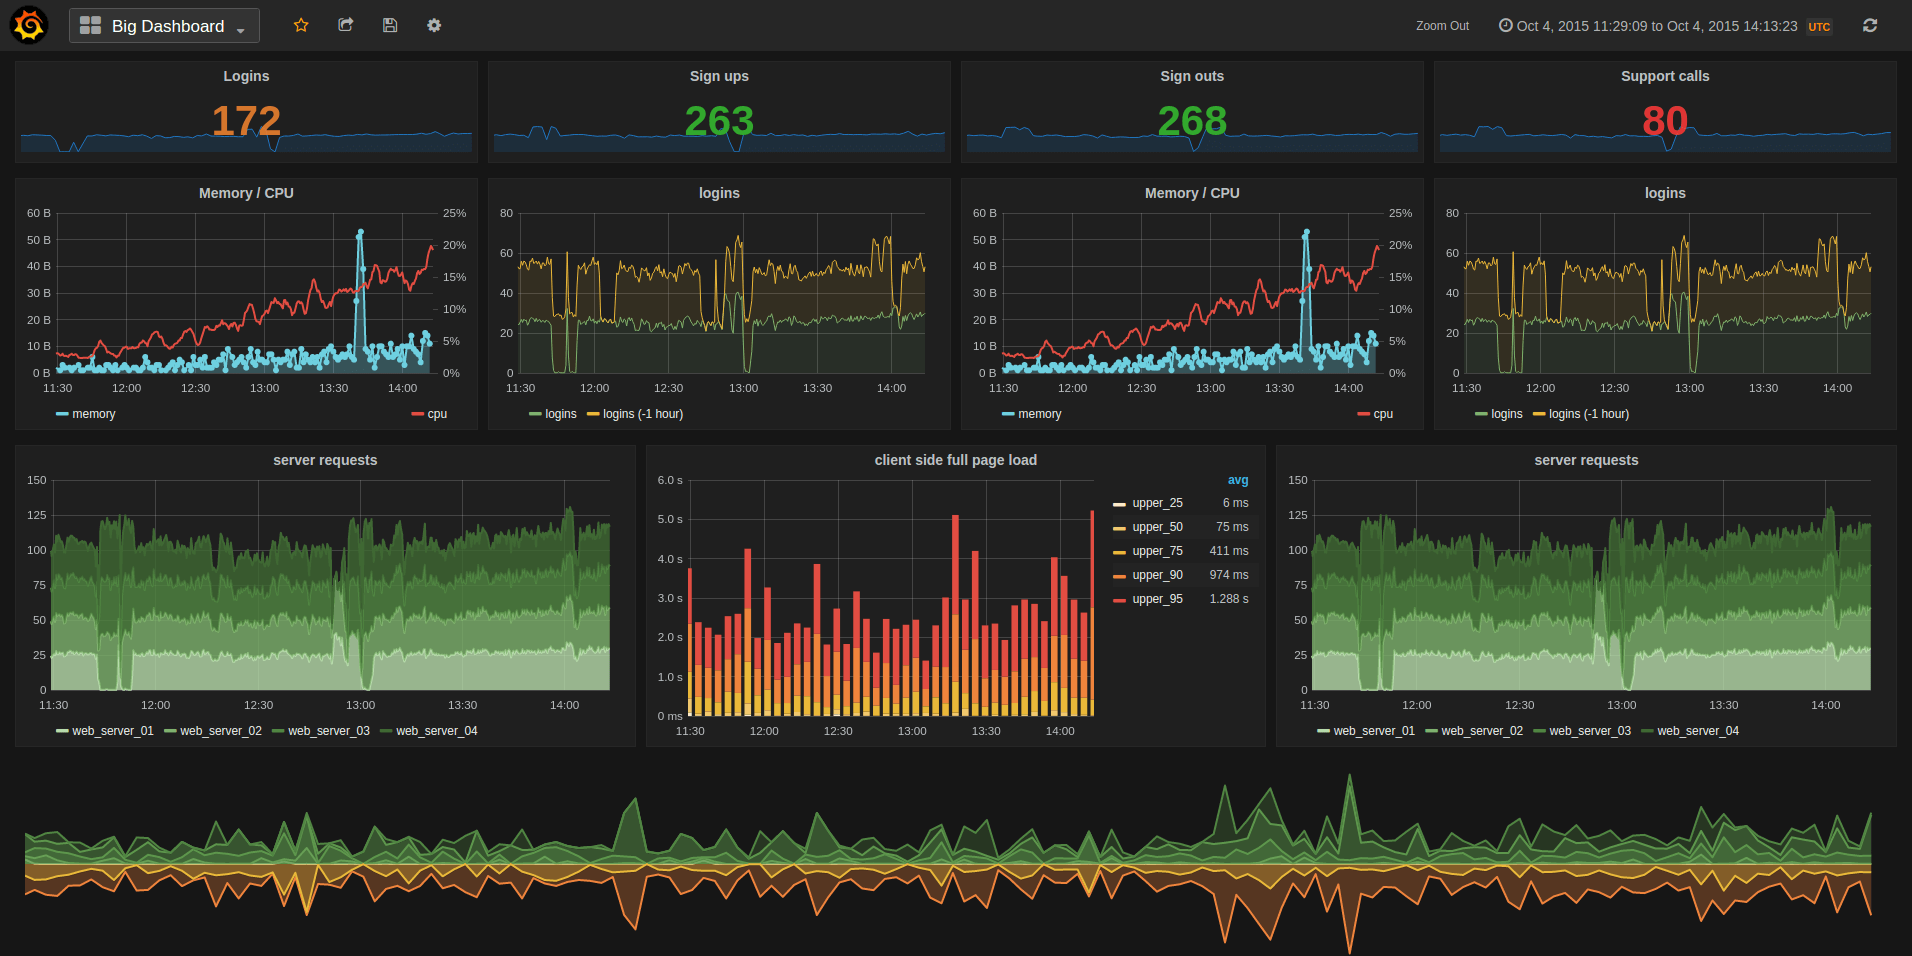
\includegraphics[scale=0.237]{dashboard_ex1}
    }
  \end{subfigure}
  \caption{Mock-up van een Grafana-dashboard}
  \label{fig:grafana}
\end{figure}

Het grootste voordeel van Grafana is dat het eenvoudig uitbreidbaar is naar andere cloud-structuren zonder al te veel wijzigingen. Daarnaast is het snel, performant en is er absolute vrijheid waar de Grafana-host zal draaien. De nadelen zijn echter de complexiteit om alles te configureren en het verplicht gebruik van Gnocchi in een OpenStack-cloud. Aangezien Gnocchi niet wordt gebruikt in de testomgeving (waar gebruik wordt gemaakt van MongoDB), biedt Grafana geen mogelijke manier om de evaluatie uit te voeren.

\subsection{Datadog}

Datadog~\cite{Datadog} is een softwarepakket in combinatie met een webapplicatie voor het monitoren van clouds. Dankzij meer dan 150 integraties van verschillende cloud-systemen zoals Amazon EC2, Kubernetes en ook OpenStack is het uitermate geschikt voor de monitoring van een cloud. Om Datadog te integreren met OpenStack moet de Datadog Agent geïnstalleerd worden op de hosts die dienst doen als hypervisor. Vervolgens kunnen er via een beveiligde omgeving op de website van Datadog online dashboards worden gecreëerd zodat er verschillende metrieken gemonitord worden. Een voorbeeld van zo'n dashboard is te zien in Figuur \ref{fig:datadog}.

\begin{figure}
  \centering
  \captionsetup{justification=centering}
  \begin{subfigure}{\textwidth}
    \centering
    \centerline{
      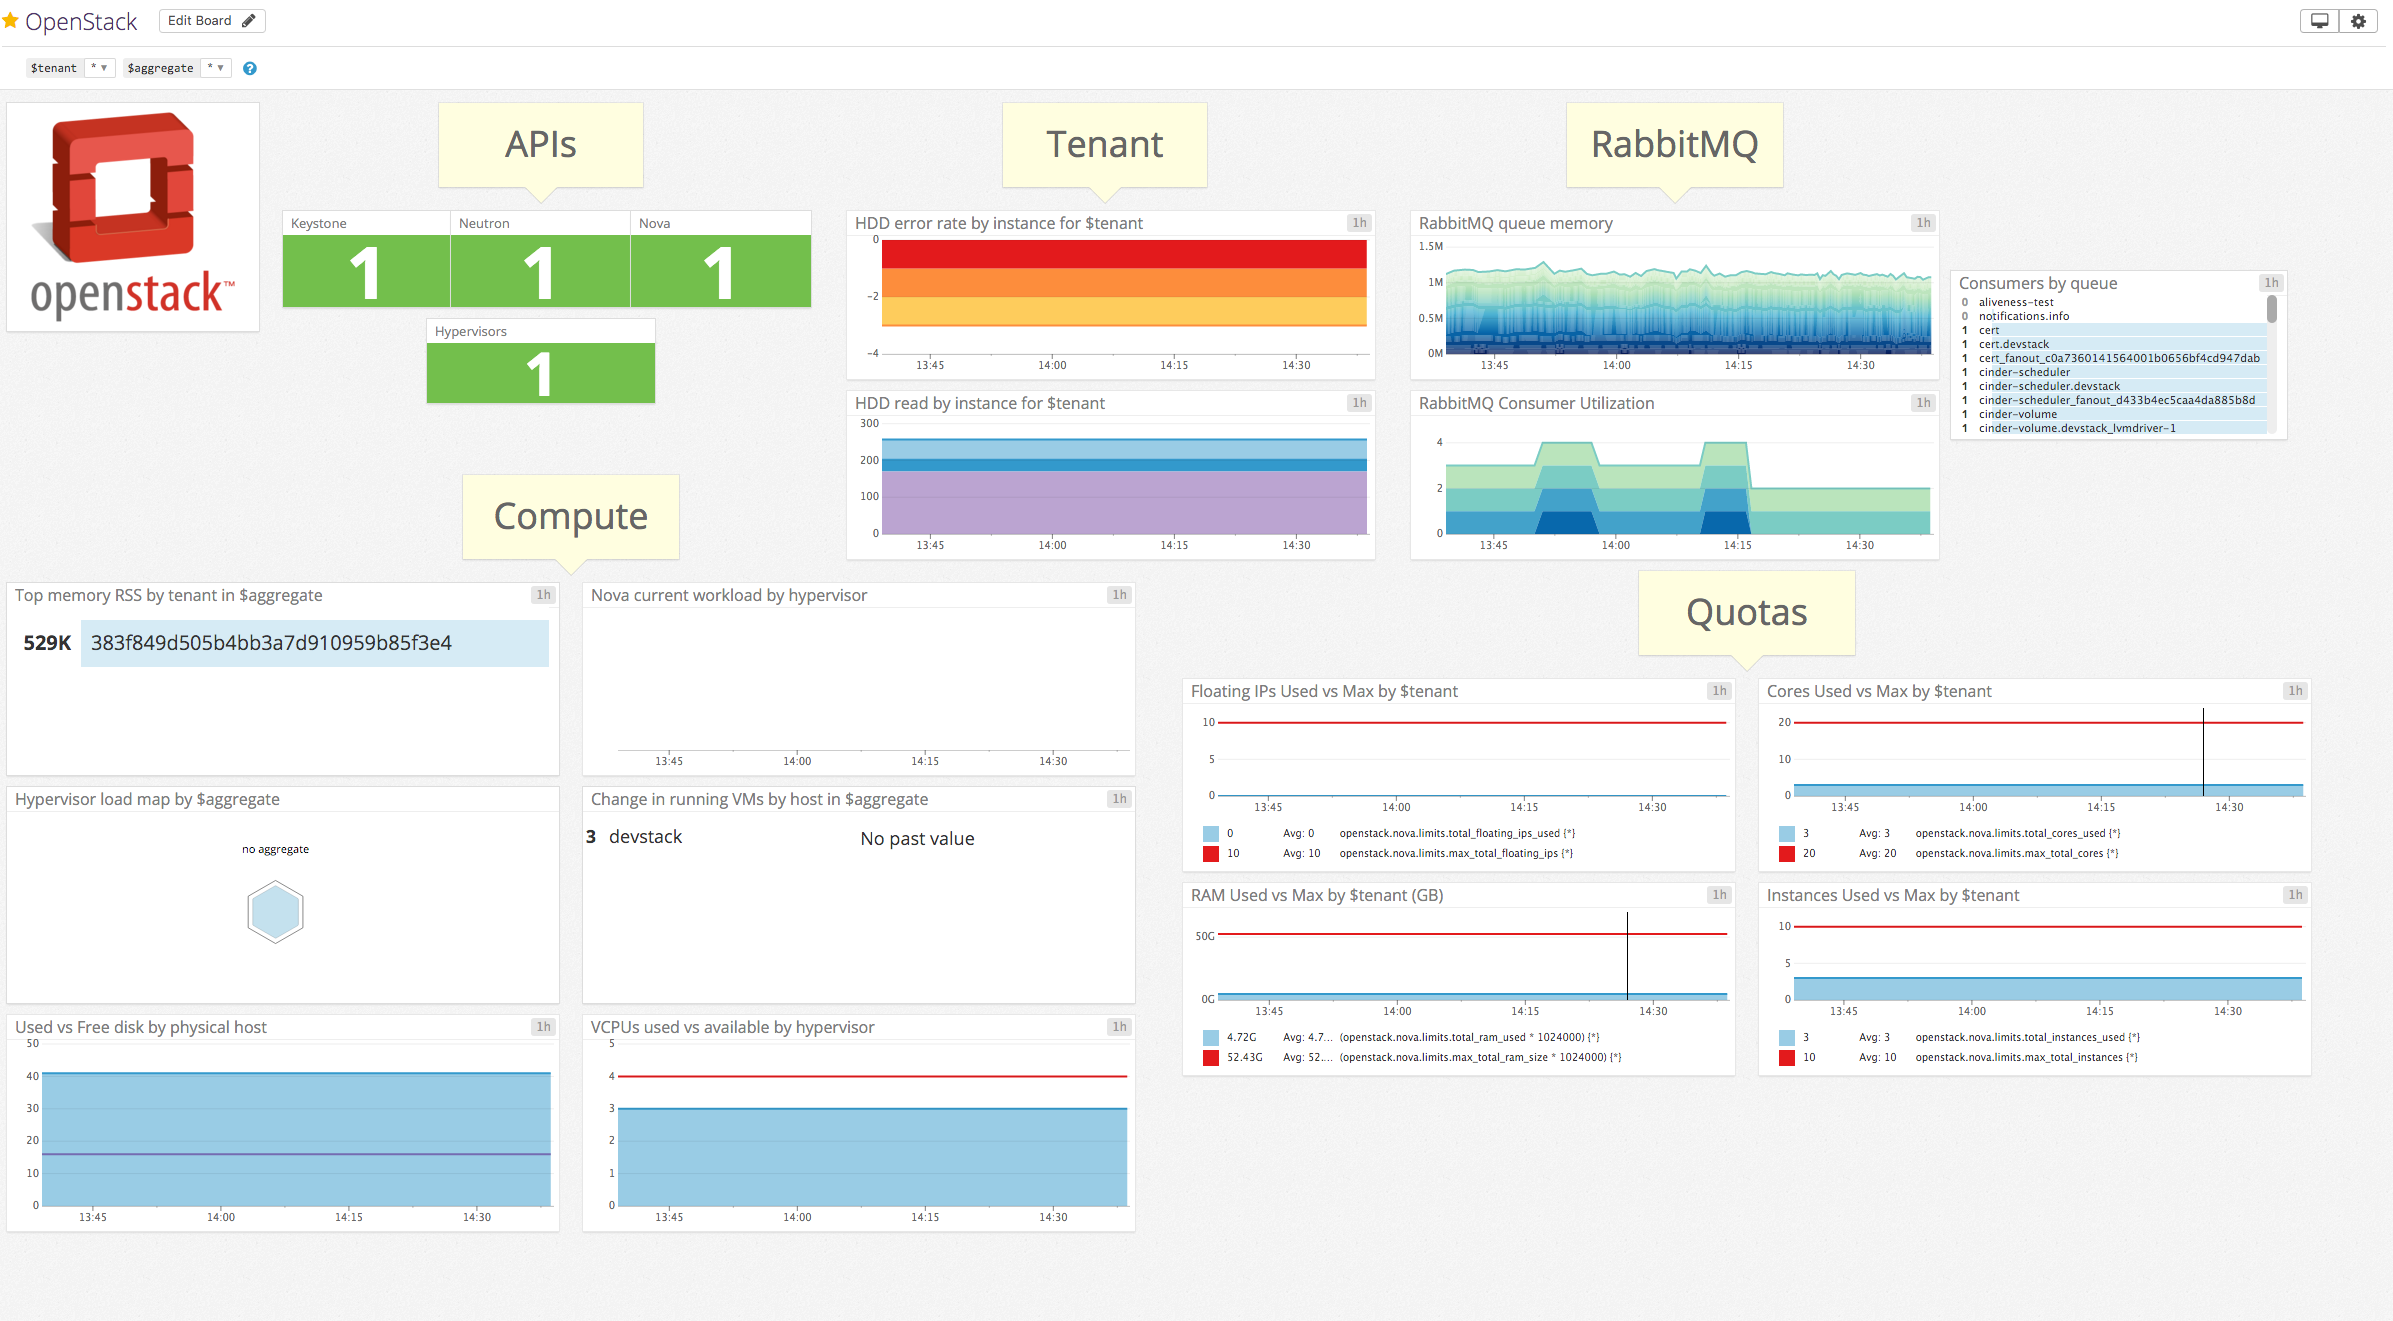
\includegraphics[scale=0.195]{datadog}
    }
  \end{subfigure}
  \caption{Mock-up van een Datadog-dashboard}
  \label{fig:datadog}
\end{figure}

Net zoals bij Grafana is het grote voordeel bij Datadog de overdraagbaarheid naar andere cloud-systemen. Daarnaast is het ook veel eenvoudiger in gebruik dankzij een eenvoudige installatie en configuratie. Datadog is beschikbaar als een gratis versie met een beperking van maximum 5 hosts waarbij enkel de standaard metrieken slechts 1 dag worden bewaard. Het grote nadeel is dat de prijs voor een beter pakket dat complexere metrieken en een langere bewaartijd biedt. Bijgevolg werd Datadog niet gekozen als optie om resource-allocatieschema's te evalueren.

\subsection{Overige mogelijkheden}

Verschillende overige mogelijkheden staan opgelijst op de monitoringpagina van OpenStack.\footnote{\url{https://wiki.openstack.org/wiki/Operations/Monitoring}} In deze lijst staan naast Rally en Datadog ook nog enkele interessante opties zoals Monasca~\cite{Openstack2017e}, een lopend OpenStack-project voor een open-source, schaalbaar, performant en fouttollerant \textit{monitoring-as-a-service} oplossing binnenin OpenStack. Andere mogelijkheden zijn bijvoorbeeld Graphite, Ganglia, Nagios, Stacktach, etc.

\section{Monitoring met Node.js en C3.js}
\label{sec:monitor_tool}

De uiteindelijke techniek om te monitoren maakt gebruik van de nodejs-agent in combinatie met een zelf ontwikkelde webapplicatie met c3.js~\cite{Tanaka2014} voor het weergeven van de grafieken. In deze sectie wordt dieper ingegaan op de nodejs-agent en de webapplicatie.

\subsection{Implementatie van de nodejs-agent}

Zoals beschreven in Sectie~\ref{sec:nodejs-agent} is de nodejs-agent een Node.js-applicatie die gebruikmaakt van verschillende node-packages. Deze applicatie is zo geschreven dat er eenvoudig nieuwe hosts kunnen worden toegevoegd of verwijderd. De code is beschikbaar via GitHub\footnote{\url{https://github.ugent.be/jfmoeyer/EvaluationRASOpenStack/tree/master/nodejs-agent}} en hier worden enkele stukken code kort toegelicht voorafgegaan door de vereisten.

Om de applicatie te kunnen starten zijn er enkele vereisten. Zo moet elke host waar de applicatie zal draaien voorzien zijn van Node.js en npm. Vervolgens moet er een MongoDB zijn die toegankelijk is voor alle hosts (eventueel met gebruikersnaam en wachtwoord). Deze databank bezit 1 tabel met de naam \textit{monitoring} en $n$ collecties waarbij $n$ staat voor het aantal hosts die gemonitord zullen worden. De databank waar Ceilometer de gegevens bewaard (in de testomgeving is dat de MongoDB op jerico-03) moet ook toegankelijk zijn voor externe verbindingen. Let wel op dat er geen authenticatie wordt ingesteld op deze databank want dit kan de werking van Ceilometer ernstig verstoren.

Een bestand dat steeds aanwezig is in een Node.js-applicatie is het package.json-bestand. Hier wordt meer informatie over de applicatie gegeven, welke commando's er uitgevoerd kunnen worden maar vooral welke afhankelijkheden (\textit{dependencies}) er nodig zijn om de geschreven code te kunnen uitvoeren. De belangrijkste afhankelijkheden hier zijn onder andere \textit{Express}, \textit{MongoDB}, \textit{Q}, etc.

Het bestand config.json bevat de nodige configuratie voor het uitvoeren van de applicatie. Hierin staan onder andere de verschillende hosts die gemonitord moeten worden, in welke tabellen de data wordt bewaard, op welke host de code wordt uitgevoerd, welke poort Express zal gebruiken, etc. In het geval van de testomgeving moest dankzij dit configuratiebestand enkel de variabele \textit{current\textunderscore host} worden aangepast per verschillende host zodat de applicatie weet op welke host hij actief is.

Systeminfo.js bevat de drie verschillende methodes die metrieken zal meten, bewaren en teruggeven. De eerste methode \textit{updateMongoDB(callback)} zal de drie metrieken, CPU-gebruik, vrij geheugen en aantal actieve instanties van de huidige host opvragen, bewaren in de MongoDB en deze ook teruggeven. De code van deze functie ziet er als volgt uit:

\begin{code}
\begin{minted}[breaklines]{javascript}
method.updateMongoDB = (callback) => {
  os.cpuUsage((cpu_usage) => {
    var free_mem = os.freemem();
    connection.query("SELECT host, count(*) from instances where power_state = 1 and host like '" + HOST_NAME + "' group by host", (error, result, fields) => {
      if (result[0]) {
        var instances = result[0]['count(*)'];
      } else {
        var instances = 0;
      }
      MongoClient.connect(url_monitoring, (err, db) => {
        assert.equal(null, err);
        insertDocument(db, cpu_usage, free_mem, instances, () => {
          db.close();
          callback({
            "cpu_usage": cpu_usage,
            "free_mem": free_mem,
            "instances": instances,
            "timestamp": new Date()
  });});});});});
}
\end{minted}
\caption{nodejs-agent: updateMongoDB-functie}
\end{code}

Als eerste wordt het CPU-gebruik berekend met behulp van de node-package \textit{os-utils}. Vervolgens wordt met hetzelfde pakket de hoeveelheid vrij geheugen opgevraagd. Daarna maakt de applicatie connectie met de MySQL-host om de hoeveelheid actieve instanties op de host te bepalen. Dit alles wordt tenslotte in de MongoDB bewaard en teruggegeven als JSON-object.

De tweede methode \textit{getPeriodStatsScale(start, end, callback)} zal de statistieken tussen een bepaalde periode (tussen start en stop) downloaden vanaf de MongoDB. De gebruikte code ziet er als volgt uit:

\begin{code}
\begin{minted}[breaklines]{javascript}
method.getPeriodStatsScale = (start, end, callback) => {
  var promises = [];
  MongoClient.connect(url_monitoring, (err, db) => {
    assert.equal(null, err);
    var complete_result = {};
    for (var node of appConfig.nodes) {
      complete_result[node.server_name + " CPU"] = [];
      complete_result[node.server_name + " Memory"] = [];
      complete_result[node.server_name + " Instances"] = [];
      var cursor = db.collection(node.mongo_table_name).find({ "timestamp": { $gt: new Date(start), $lt: new Date(end) } });
      var promise = new Promise((resolve, reject) => {
        var node_name = node.server_name;
        cursor.each((err, doc) => {
          if (err) {
            reject("Something went wrong with node " + node_name);
          }
          if (doc != null) {
            complete_result[node_name + " CPU"].push(doc.cpu_usage);
            complete_result[node_name + " Memory"].push(doc.free_mem);
            complete_result[node_name + " Instances"].push(doc.instances);
          } else {
            resolve(node_name + " is inserted!");
      }});});
      promises.push(promise);
    }
    Q.all(promises).then(() => {
      db.close();
      callback(complete_result);
    }).fail(console.error);
  });
}
\end{minted}
\caption{nodejs-agent: getPeriodStatsScale-functie}
\end{code}

De belangrijkste functionaliteit van deze functie is het gebruik van Promises binnen JavaScript. Dit laat namelijk toe dat indien er een connectie is met de MongoDB, elke node uit het conf.json-bestand overlopen wordt en dit bepaalde methodes zal uitvoeren (zoals alle metrieken opvragen). Vervolgens zal dankzij het node-package \textit{Q} gewacht worden totdat alle Promises voltooid zijn waarna het verkregen resultaat kan worden teruggegeven.

De laatste methode om metrieken op te vragen is \textit{getCeilometerAndInstancesTimeScale(start, stop, callback)}. Deze dient om de werklast, gemeten door Ceilometer, op te vragen samen met het aantal instanties per host. De gebruikte code ziet er uit als volgt:

\begin{code}
\begin{minted}[breaklines]{javascript}
method.getCeilometerAndInstancesTimeScale = (start, stop, callback) => {
  MongoClient.connect(url_ceilometer, (err, db) => {
    assert.equal(null, err);
    var cursor = db.collection("meter").find({ timestamp: { $gt: new Date(start), $lt: new Date(stop) }, counter_name: appConfig.scale_app.counter_name, "resource_metadata.display_name": appConfig.scale_app.scale_group_name, "resource_metadata.status": "active" });
    var result = {};
    var complete_result = {};
    var promises = [];
    cursor.each((err, doc) => {
      if (doc != null) {
        result[doc.timestamp] = doc.counter_volume;
      } else {
        db.close();
          MongoClient.connect(url_monitoring, (err, db) => {
            assert.equal(null, err);
            for (var node of appConfig.nodes) {
              complete_result[node.server_name] = {};
              var cursor = db.collection(node.mongo_table_name).find({ "timestamp": { $gt: new Date(start), $lt: new Date(stop) } });
              var promise = new Promise((resolve, reject) => {
                var node_name = node.server_name;
                cursor.each((err, doc) => {
                  if (err) {
                    reject("Something went wrong with node " + node_name)
                  }
                  if (doc != null) {
                    complete_result[node_name][doc.timestamp] = doc.instances;
                  } else {
                    resolve(node_name + " is inserted!");
              }});});
            promises.push(promise);
            }
          Q.all(promises).then(() => {
            db.close();
            callback([result, complete_result]);
          }).fail(console.error);
  });}});});
}
\end{minted}
\caption{nodejs-agent: getCeilometerAndInstancesTimeScale-functie}
\end{code}

Hier wordt eveneens gebruikgemaakt van Promises om alle hosts in het configuratiebestand te overlopen. Eerst worden de gegevens van de ceilometer-databank opgevraagd en nadien de metrieken van elke host. Op het einde van de code wordt er gewacht tot alle Promises zijn voltooid alvorens het resultaat wordt teruggegeven aan de callback-functie.

Het laatste bestand in deze applicatie heet \textit{rpicluster.agent.js}. Dit is het kloppend hart van de applicatie doordat deze de aanvragen vanuit de buitenwereld zal verwerken en uitvoeren. Met behulp van het Express-package van Node wordt er een router geïnitialiseerd, geconfigureerd en per aanvraag, zoals vermeld in Sectie~\ref{sec:nodejs-agent}, een functie geïmplementeerd. Een voorbeeld van zulke functie ziet er uit als volgt:

\begin{code}
\begin{minted}[breaklines]{javascript}
router.get("/timestats", function(req, res) {
  res.writeHead(200, { 'Content-Type': 'application/json'});
  var url_parts = url.parse(req.url, true);
  var query = url_parts.query;
  new Systeminfo().getCeilometerAndInstancesTimeScale(query.start, query.stop, (result) => {
    res.end(JSON.stringify(result));
  });
});
\end{minted}
\caption{nodejs-agent: nodejs-agent: implementatie van een aanvraag}
\end{code}

Vooraleer deze code tot stand is gekomen, werd er eerst gebruik gemaakt van asynchrone en hard-coded aanvragen die moeilijk uit te breiden waren naar meer of minder hosts. Dankzij de overschakeling naar het gebruik van Promises en het conf.json-bestand, zijn er twee voordelen. Er kunnen eenvoudig meerdere hosts worden toegevoegd of verwijderd (de databank die alles bewaard kan zelfs extern zijn) en dankzij het gebruik van de Promises is de code performanter omdat deze stukken code ``gelijktijdig'' uitgevoerd worden.

Om de nodejs-agent te starten zijn er slechts twee commando's nodig, één om de nodige afhankelijkheden te installeren en één om de applicatie te starten. De twee commando's, waarbij de \& in het laatste commando ervoor zorgt dat de applicatie in de achtergrond wordt uitgevoerd, zijn de volgende:

\begin{code}
\caption{Starten van de nodjs-agent}
\begin{minted}[breaklines]{bash}
$ sudo npm install
$ sudo npm start &
\end{minted}
\end{code}

\subsection{Implementatie van de webapplicatie}

De webapplicatie bestaat uit twee pagina's, één voor live-monitoring en één voor het opvragen van gegevens die gemeten zijn tijdens een bepaalde periode (op voorwaarde dat er tijdens die periode live-monitoring is gebeurd). Ze werkt nauw samen met de nodejs-agent voor het opvragen van gegevens en het aansturen van de databank. Ook in de webapplicatie werd gebruikgemaakt van een configuratiebestand zodat er eenvoudig meerdere hosts kunnen worden toegevoegd of verwijderd. De code is beschikbaar via GitHub\footnote{\url{https://github.ugent.be/jfmoeyer/EvaluationRASOpenStack/tree/master/webapp}} en maakt gebruik van c3.js~\cite{Tanaka2014} voor het visualiseren van de grafieken. Ook hier worden Promises gebruikt voor zowel betere performantie als schaalbaarheid. Aangezien de code zeer gelijkaardig is aan die van de nodejs-agent wordt deze hier ook niet verder besproken.

De live-monitoring pagina wordt weergegeven in Figuur~\ref{fig:webapp1} en Figuur~\ref{fig:webapp2} en de functionaliteiten worden hier kort besproken. De drie grafieken in deelfiguur (a) geven respectievelijk het CPU-gebruik, de hoeveelheid vrij geheugen en het aantal actieve instanties weer per host. Indien de gebruiker de grafieken wenst te verbergen tijdens een sessie, kan hij deze uitschakelen en zal een spinner aangeven of het monitoren bezig is of niet wat te zien is in deelfiguur (b). Bij een sessie zal er standaard elke 2 seconden (2000 ms) een aanvraag worden gestuurd naar de nodejs-agent voor het bewaren en teruggeven van de metrieken op dat moment (de /mongodb aanvraag van de nodejs-agent). Het interval kan aangepast worden naar belangen van de gebruiker. Vooraleer het monitoren kan gestart worden, is er een controle of de te monitoren hosts wel beschikbaar zijn. Dit gebeurt via een ping-aanvraag naar alle hosts en pas wanneer alle hosts antwoord geven, kan er gemonitord worden.

\begin{figure}
\centering
\subcaptionbox{Live monitoring - grafieken zichtbaar \label{fig:webapp1}}{%
  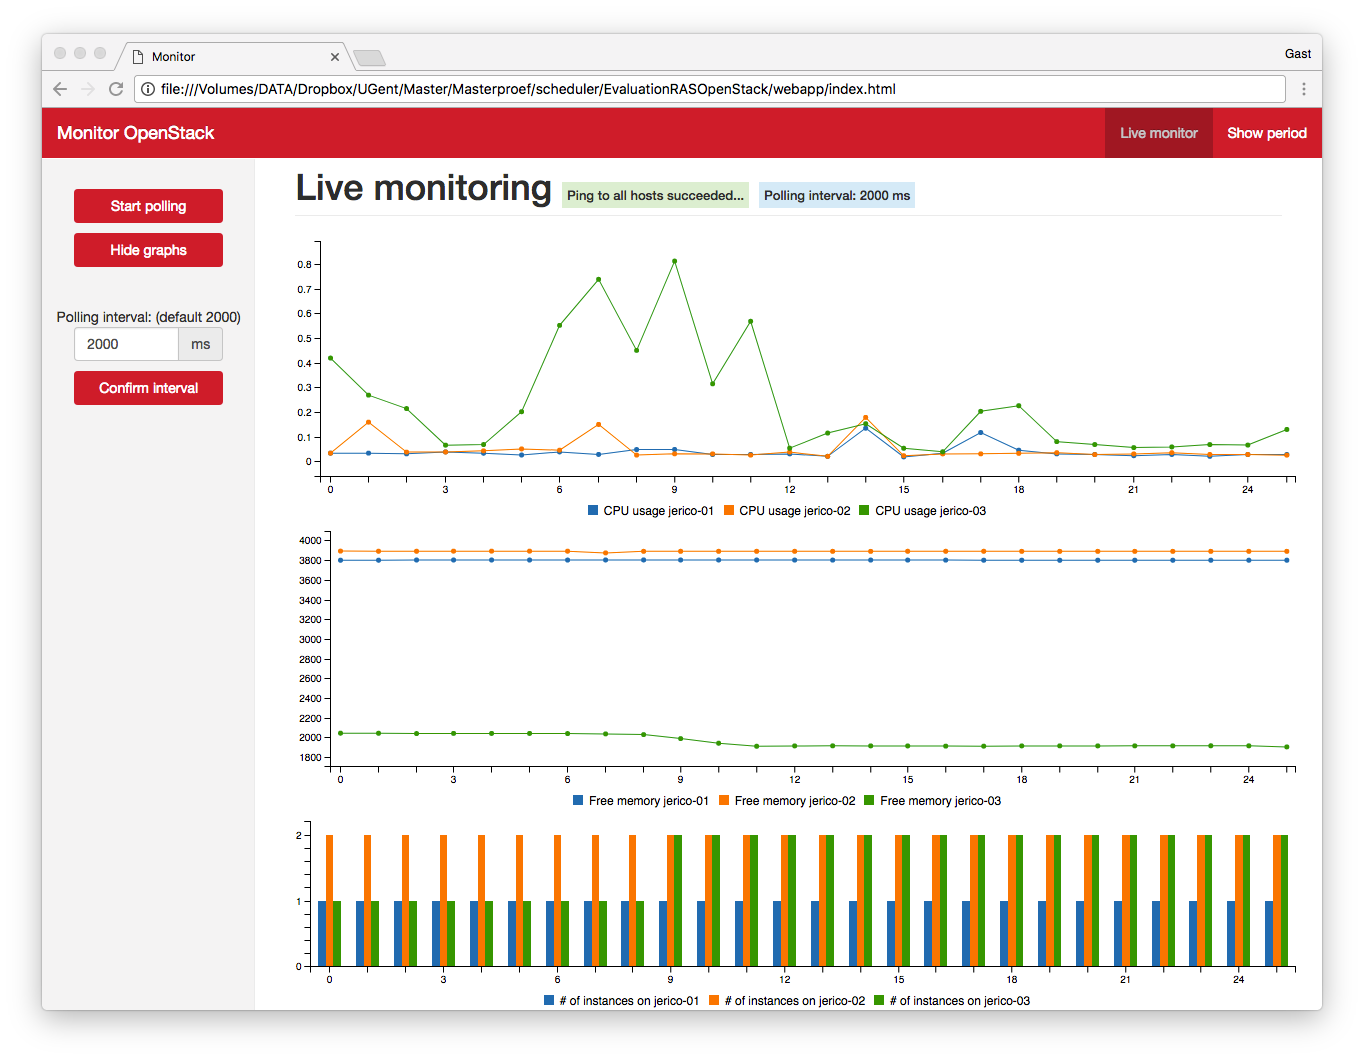
\includegraphics[width=0.65\textwidth]{webapp_img1}%
}\par\medskip
\subcaptionbox{Live monitoring - grafieken verborgen \label{fig:webapp2}}{%
  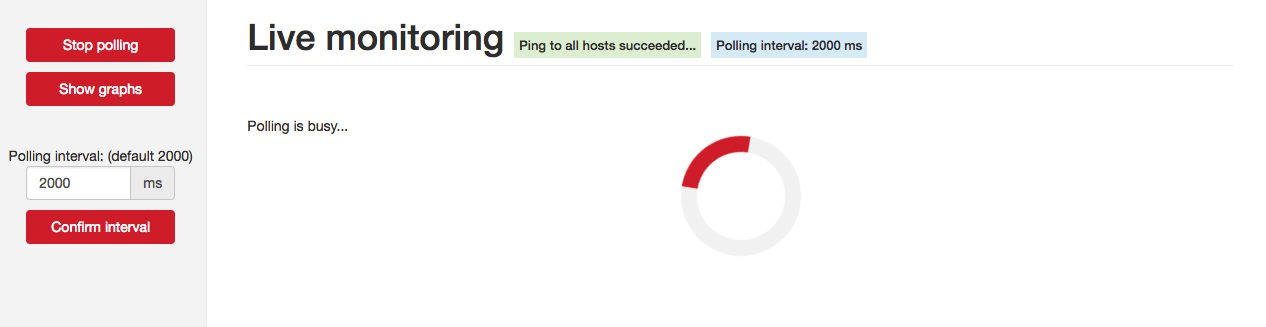
\includegraphics[width=0.65\textwidth]{webapp_img2}%
}\par\medskip
\subcaptionbox{Overzicht van een periode \label{fig:webapp3}}{%
  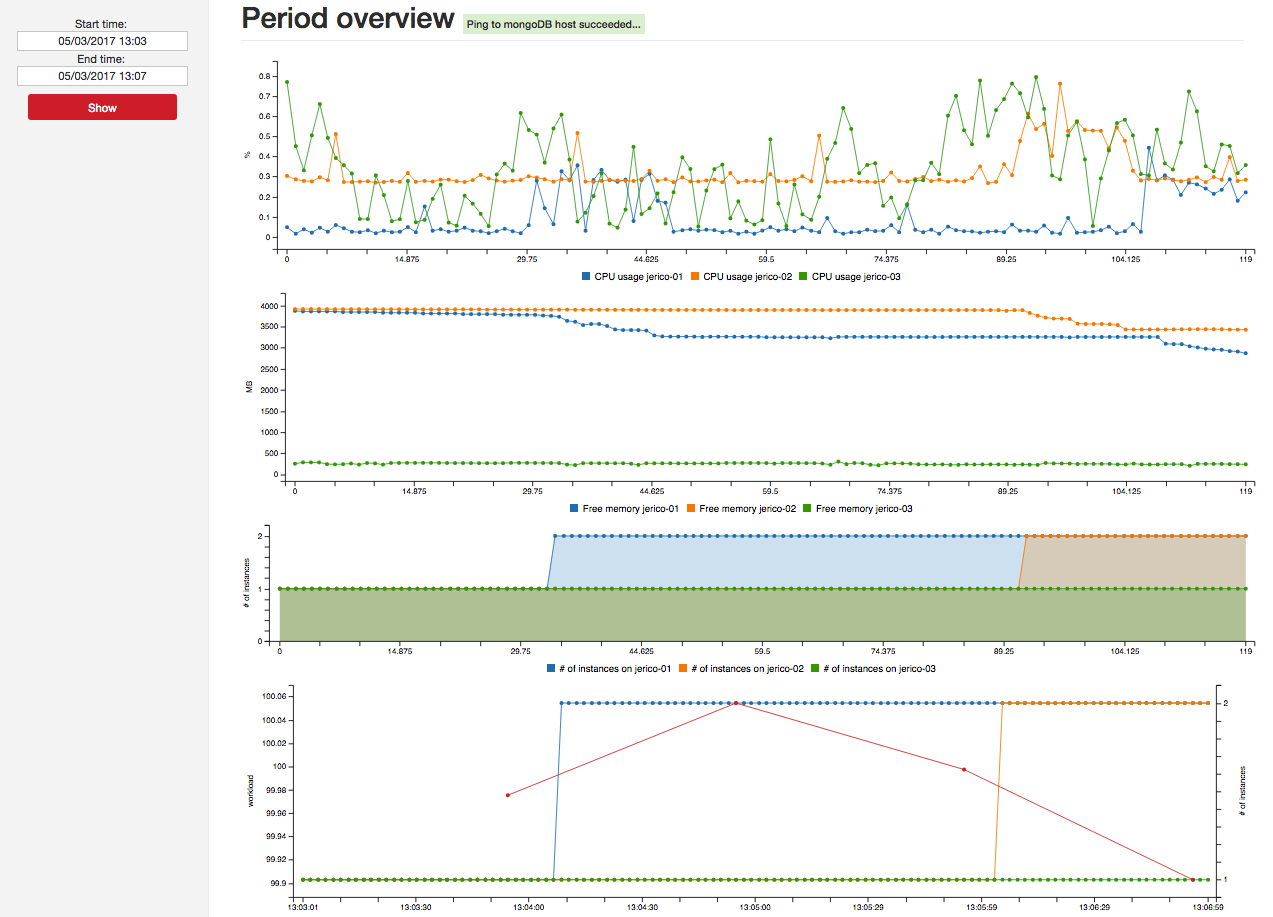
\includegraphics[width=0.65\textwidth]{webapp_img3}%
}
\caption{Webapplicatie}
\label{fig:webapp}
\end{figure}

De periode-pagina wordt weergegeven in Figuur~\ref{fig:webapp3} en is zeer gelijkaardig aan de live-monitor pagina. Hier wordt wel een extra grafiek weergegeven, die het aantal instanties per host combineert met de gemeten statistieken van Ceilometer. Onmiddellijk na het laden van de pagina wordt er gecontroleerd of de host die de databank bevat bereikbaar is. Enkel indien deze bereikbaar is kan er een periode worden ingevoerd en zal deze gevisualiseerd worden in de 4 grafieken.

%\chapter{Evaluatie van resource allocatieschema's}
\label{chap:evaluation}

In dit hoofdstuk wordt de eigenlijke Proof-of-Concept besproken en geëvalueerd. Met behulp van de testomgeving, beschreven in Hoofdstuk~\ref{sec:environment} en de monitor tools, uitgelegd in Hoofdstuk~\ref{chap:monitoring} is de hele evaluatie uitgevoerd.

De opbouw van dit hoofdstuk is als volgt. Eerst wordt er uitgelegd hoe de FaaFo-applicatie werklast kan genereren op één of meerdere worker-instanties. Vervolgens wordt een korte hypothese beschreven met het verwachte resultaat van de werking van Round Robin. Nadien wordt een test uitgevoerd met Rally om te bekijken of het schema naar behoren werkt op high-level niveau om af te sluiten met een stress-test, die wordt gemonitord en besproken.

\section{De schaalbare FaaFo-applicatie}
\label{sec:scalable_faafo}

Zoals besproken in Sectie~\ref{sec:faafo} is de FaaFo-applicatie uitermate geschikt om een stress-test uit te voeren op de drie gebruikte hypervisors met de RoundRobinScheduler ingeplugd in Nova. Na het activeren van de OpenStack stack kan er via de FaaFo-controller een commando worden ingegeven die voor voldoende werklast zal zorgen. De OpenStack-Orchestration en -Telemetry services laten dan alarmen afgaan bij een hoge werklast waardoor er extra worker-instanties aangemaakt worden. Zoals beschreven in de template in Sectie~\ref{sec:faafo_template} kunnen er maximum zeven worker-instanties tegelijkertijd actief zijn.

Op de OpenStack controller-node, jerico-03, kan dankzij de security group instellingen en de gebruikte sleutel (de key\textunderscore name parameter) een SSH-verbinding gelegd worden met de FaaFo-controller. Van hieruit kunnen er dan verschillende taken gestart worden als ook het weergeven van de huidige taken. De FaaFo-applicatie is zo gemaakt dat deze met volgende simpele commando's kan werken:

\begin{code}
\begin{minted}[breaklines]{bash}
$ faafo create --width 5555 --height 5555 --tasks 3
$ faafo list
\end{minted}
\caption{Starten van drie FaaFo-taken}
\end{code}

Het eerste commando zal 3 taken creëren die elk een fractaal moeten berekenen van de meegegeven hoogte en breedte. Deze drie taken komen dan terecht in de queue op FaaFo-controller waarna de FaaFo-workers een taak van de queue halen en deze uitvoeren. Het berekenen van een fractaal vergt veel CPU-verbruik en hierdoor zal het \textit{cpu\textunderscore alarm\textunderscore high}-alarm getriggerd worden. De OpenStack Orchestration-services, Heat, zullen hierop reageren door extra FaaFo-workers aan te maken.

Het tweede commando geeft een overzicht weer van de berekende en nog te berekenen fractalen, telkens met hun afmetingen en hun grootte op de harde schijf. Is de grootte nog nul, dan betekent dit dat het fractaal nog berekend moet worden, of dat er een FaaFo-worker mee bezig is

\section{Hypothese}

Round Robin is een contextloos algoritme, het weet niets af van de hosts hun capaciteiten. Bijgevolg wordt er verwacht dat de Rally-test een gunstig resultaat zal afleveren omdat deze test ook zonder context wordt uitgevoerd. Het gewoon starten en stoppen van instanties zonder generatie van werklast is ideaal voor een Round Robin schema en bijgevolg zullen alle instanties gelijkmatig verdeeld worden over de verschillende hosts.

In het geval van de schaalbare FaaFo-applicatie kunnen de nadelen van een Round Robin schema wel eens zichtbaar worden. De Orchestration-services van OpenStack verwijderen immers een willekeurige host bij een laag-cpu-alarm. Indien er nadien terug instanties bijkomen door een hoog-cpu-alarm, kan het zijn dat een host meer instanties bevat dan andere waardoor de werklast niet gelijk verdeeld zal worden.  In welke mate dit nadelig is, zal de test zelf moeten aantonen.

\section{Evaluatie met Rally}

De evaluatie met Rally gebeurt met dezelfde template zoals beschreven in Sectie~\ref{sec:rally}. Het enige verschil met de test die daar is uitgevoerd, is de gebruikte Nova-scheduler. De resultaten van de test zijn te zien in Figuur~\ref{fig:evaluation_rally}. De bovenste grafiek is de uitvoer van Rally zelf, gelijkaardig aan het resultaat uit Sectie~\ref{sec:rally}, de onderste grafiek is de uitvoer van de zelf ontwikkelde monitorapplicatie beschreven in Sectie~\ref{sec:monitor_tool}.

Zoals verwacht in de hypothese wordt de Rally-test beëindigd zonder fouten. Dit komt omdat de instanties steeds gelijkmatig worden verdeeld over de drie hosts. Dit is ook te zien in de Figuur~\ref{fig:evaluation_rally2} waarbij geen enkele host meer dan 2 instanties tegelijkertijd bezit. Verrassend aan het resultaat is dat de RoundRobin-scheduler er duidelijk langer over doet om alles te starten en te stoppen vergeleken met Figuur~\ref{fig:rally-test1} en Figuur~\ref{fig:rally-test2}. Doordat tegelijkertijd de nodejs-agent op de hosts data aan het verzamelen was, kan dit een mogelijke verklaring zijn voor de iets langere duurtijd.

Uit deze test kunnen volgende besluiten genomen worden. Omdat deze test contextloos is (er werd nergens werklast gegenereerd), werkt een RoundRobin-scheduler naar behoren. De werklast op de host jerico-03 is wel een pak groter dan die op de andere hosts. Een mogelijke verklaring hiervoor is het feit dat jerico-03 zowel de OpenStack-controller is en dus de andere hosts moet aansturen alsook zelf instanties moet hosten. Daarom is het aan te raden om een OpenStack-controller geen dienst te laten doen als hypervisor, zodat de werklast beter verdeeld kan worden.

\begin{figure}
	\centering
	\subcaptionbox{Uitvoer van Rally \label{fig:evaluation_rally1}}{%
		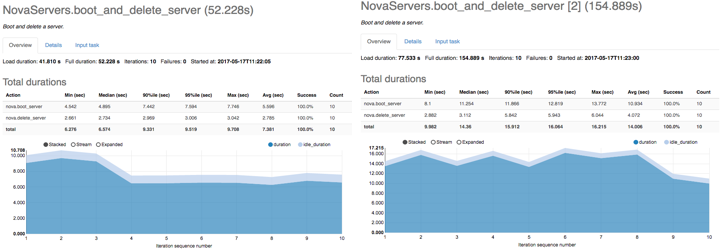
\includegraphics[width=1.00\textwidth]{Dia3}%
	}\par\medskip
	\subcaptionbox{Uitvoer van de monitorapplicatie \label{fig:evaluation_rally2}}{%
		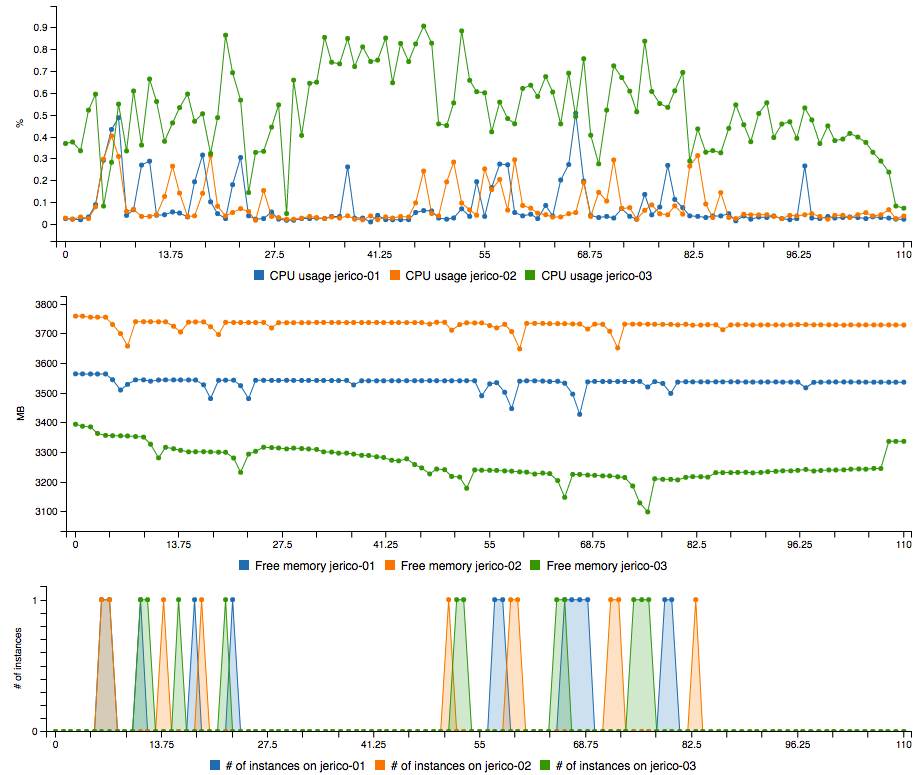
\includegraphics[width=1.00\textwidth]{rally_evaluation}%
	}
	\caption{Evaluatie met Rally - Resultaten}
	\label{fig:evaluation_rally}
\end{figure}

\section{Evaluatie met de FaaFo-applicatie}
\begin{figure}
	\centering
	\captionsetup{justification=centering}
	\begin{subfigure}{\textwidth}
		\centering
		\centerline{
			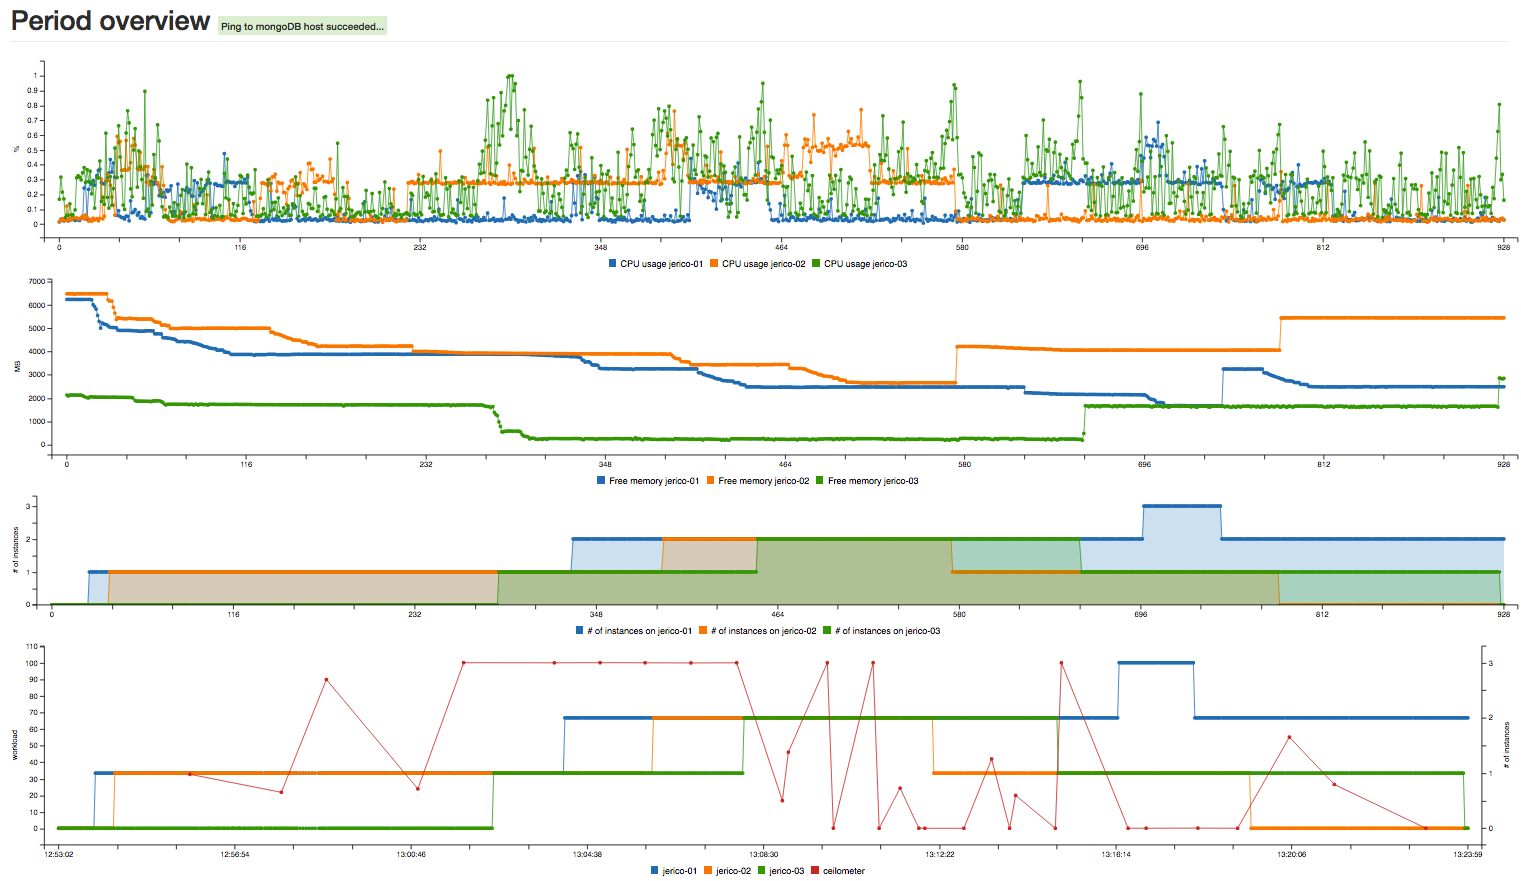
\includegraphics[width=\textwidth]{faafo_evaluation}
		}
	\end{subfigure}
	\caption{Resultaat van de stress-test met de FaaFo-applicatie}
	\label{fig:evaluation_faafo}
\end{figure}

Het Round Robin schema wordt ook getest met de schaalbare FaaFo-applicatie. De gemeten resultaten met de nodejs-agent bedekken de hele procedure, vanaf het creëren van de stack tot en met het voltooien van het \textit{faafo create}-commando en deze worden weergegeven in Figuur~\ref{fig:evaluation_faafo}.

Ook hier komen de resultaten goed overeen met de verwachte hypothese. De instanties worden in het begin evenredig verdeeld over de verschillende hosts. Ongeveer halverwege de resultaten zijn er enkele metingen met een laag cpu-gebruik, waardoor enkele worker-instanties verwijderd worden. Nadien worden terug hoge waarden gemeten van het cpu-gebruik waardoor nieuwe worker-instanties worden gestart. Deze nieuwe worker-instanties worden geplaatst op de eerstvolgende host in de rij van het Round Robin schema, zonder dat deze rekening houdt met de verwijderde instanties. Hierdoor zijn de instanties naar het einde van de test toe niet meer evenredig verdeeld en dat is ook zichtbaar in de derde en vierde grafiek.

Net zoals bij de Rally-test is de werklast op de OpenStack-controller groter dan bij de andere hosts. Ook de hoeveelheid vrij geheugen is beperkt op de OpenStack-controller in vergelijking met de andere hosts. In een worst-case scenario kan het zijn dat de instanties verwijderd worden op alle hosts met uitzondering van jerico-03, waardoor de hoeveelheid vrij geheugen op deze host te laag is om nog een nieuwe instantie te hosten. Indien de volgende nieuwe instantie dan net op jerico-03 gehost wordt, zorgt dit voor ernstige gevolgen zoals bijvoorbeeld het uitvallen van jerico-03 en dus de gehele OpenStack-omgeving.


\section{Resultaat van de evaluaties}

Een Round Robin schema is simpel en werkt naar behoren in de meeste gevallen. Het grootste nadeel is de contextloze eigenschap van dit schema waardoor er mogelijks problemen optreden bij een tekort aan fysieke resources. De gestelde hypothese voorafgaand aan de verschillende evaluaties is zeer aansluitend aan de verkregen resultaten mits het toevoegen van enkele bijkomende conclusies.

Door het hele proces te overlopen, vanaf het opzetten van de testomgeving tot de verschillende evaluaties, werd de Proof-of-Concept aangetoond. Het grootste deel van de gebruikte configuratie en code kan herbruikt worden bij andere allocatieschema's. Enkel het nieuwe schema moet worden geschreven in Python met de nodige overerving van de Nova-filters. Na die aanpassing is het mogelijk om het gehele evaluatieproces opnieuw te overlopen om zo de resultaten te bekomen, die nodig zijn voor de evaluatie van het nieuwe schema.


%\chapter{Conclusie}

De bedoeling van deze thesis is het aanbieden van een eenvoudig en relatief snelle methode om nieuwe cloud-allocatieschema's te evalueren op een echt OpenStack-testbed. Zoals beschreven in het gerelateerd werk in Hoofdstuk~\ref{chap:rel_work}, is er de laatste tijd veel onderzoek gebeurd naar nieuwe cloud resource-allocatieschema's. Deze nieuwe schema's werden in de meeste gevallen getest en geëvalueerd op een simulator in plaats van op een fysiek cloud-testbed. Een belangrijke reden voor het gebruik van een simulator in plaats van een fysiek cloud-testbed is de kostprijs en de vereiste configuratie. In deze thesis kan er, met behulp van DevStack, snel en eenvoudig een OpenStack-cloud worden uitgerold op een fysiek cloud-testbed. Het voordeel van OpenStack is dat het een gratis softwarepakket is, compatibel met relatief goedkope hardware. Dankzij DevStack valt er veel configuratie weg en daarmee worden de twee grote redenen om geen fysiek cloud-testbed te gebruiken vermeden. Het te testen allocatieschema moet ``vertaald'' worden zodat het kan samenwerken met Nova, een OpenStack onderdeel verantwoordelijk voor het zware rekenwerk. Deze samenwerking tussen het te testen allocatieschema en Nova kan, dankzij de open-source code van OpenStack, eenvoudig gebeuren, mits enkele aanpassingen. Na het inpluggen van dat nieuwe schema kan er via de template een schaalbare applicatie worden uitgerold op de cloud. Deze schaalbare applicatie zorgt voor echte werklast op de fysieke hypervisors door het berekenen van enkele complexe fractalen waardoor de applicatie kan in- en uitgeschaald worden door de OpenStack-componenten Heat, Ceilometer en Aodh. De monitorapplicatie bewaakt dit gehele proces en bewaart statistieken in een databank. Nadien kunnen deze statistieken worden opgevraagd zodat dit alles kan geëvalueerd worden.

Om dit alles te bewijzen is er gedurende deze thesis een Proof-of-Concept uitgewerkt met een Round-Robin allocatieschema. De resultaten hiervan worden besproken in Hoofdstuk~\ref{chap:evaluation} en zijn zoals verwacht aansluitend bij de gestelde hypothese. Round Robin is een simpel allocatieschema dat in sommige contexten zeer bruikbaar is, maar het grote nadeel blijft dat het volledig contextloos werkt.

Het eigenlijke besluit van deze thesis luidt dat via OpenStack uitgerold met behulp van DevStack, de schaalbare FaaFo-applicatie, Rally en de monitortechniek er een nieuw schema kan worden uitgetest en geëvalueerd. Het enige dat nog dient te gebeuren is het nieuwe schema inpluggen in Nova en deze service herstarten.
\bibliographystyle{ieeetr}
\bibliography{referenties}

%\begin{appendices}
\section*{Bijlage A - OpenStack's installatiehandleiding}
\label{att:installation}

Hier wordt een overzicht gegeven van de installatie van OpenStack met behulp van DevStack (commit 	713f17c1d29f097d7d65e243c97a026867bf9363\footnote{\url{https://git.openstack.org/cgit/openstack-dev/devstack/commit/?id=713f17c1d29f097d7d65e243c97a026867bf9363}}) op een controller node en twee compute nodes.~\cite{DevStack2017}~\cite{DevStack2017a}~\cite{AskUbuntu2011} De drie nodes zijn elk voorzien van 10 GB HDD, 8 GB vRAM en 2 vCPU's. Als standaard besturingssysteem wordt Ubuntu Server 16.04.02 LTS gebruikt.

\subsubsection{Controller node}

\begin{code}
\begin{minted}[breaklines]{bash}
$ sudo apt-get update
$ cd /
$ sudo git clone https://git.openstack.org/openstack-dev/devstack
$ cd devstack/
$ sudo cp samples/local.conf local.conf
$ sudo vi local.conf
\end{minted}
\end{code}

In local.conf plaatst men volgende gegevens:

\begin{code}
\begin{minted}[breaklines]{bash}
[[local|localrc]]
	HOST_IP=192.168.16.118
	FLAT_INTERFACE=ens160
	FIXED_RANGE=10.4.128.0/20
	FIXED_NETWORK_SIZE=4096
	FLOATING_RANGE=192.168.16.128/25
	MULTI_HOST=1
	ADMIN_PASSWORD=CaHiBaPa
	DATABASE_PASSWORD=CaHiBaPa
	RABBIT_PASSWORD=CaHiBaPa
	SERVICE_PASSWORD=CaHiBaPa

	enable_service placement-api
	enable_service placement-client

	disable_service n-net
	enable_service q-svc
	enable_service q-agt
	enable_service q-dhcp
	enable_service q-l3
	enable_service q-meta
	enable_service neutron
	enable_service n-novnc #Automatisch geactiveerd sinds 13 maart 2017

	enable_plugin heat https://git.openstack.org/openstack/heat

	CEILOMETER_BACKEND=mongodb
	enable_plugin ceilometer https://git.openstack.org/openstack/ceilometer
	enable_plugin aodh https://git.openstack.org/openstack/aodh
	CEILOMETER_PIPELINE_INTERVAL=60
	CEILOMETER_NOTIFCATION_TOPICS=notifications,profiler
\end{minted}
\end{code}

\begin{code}
\begin{minted}[breaklines]{bash}
$ sudo vi stackrc
	//Wijzig de GIT_BASE van git:// naar https://
$ sudo /devstack/tools/create-stack-user.sh
$ sudo chown -R stack:stack /devstack
$ sudo su stack
$ /devstack/stack.sh
\end{minted}
\end{code}

De installatie zelf zal ongeveer een halfuur tot een uur in beslag nemen. Na de installatie geeft DevStack een overzicht van de gebruikers, de wachtwoorden en de URL's naar het dashboard en de identity service.
\\
Een belangrijke en goede eigenschap van DevStack is dat het de verschillende OpenStack services start en monitort in verschillende terminals. Bij het gebruik van een SSH-connectie naar de controller node is het interessant dat ook deze schermen beschikbaar zijn voor eventuele debuginformatie of het heropstarten van bepaalde services. Hiervoor moet volgend commando uitgevoerd worden:

\begin{code}
\begin{minted}[breaklines]{bash}
$ sudo chown stack:stack `readlink /proc/sefl/fd/0`
\end{minted}
\end{code}

Dit commando geeft de stack-gebruiker toegang tot de verschillende terminals waardoor er eenvoudig via onderstaand commando verwisselt kan worden tussen de verschillende schermen, ook wel \textit{screens} genaamd.

\begin{code}
\begin{minted}[breaklines]{bash}
$ screen -x stack
\end{minted}
\end{code}

\subsubsection{Compute nodes}

\begin{code}
\begin{minted}[breaklines]{bash}
$ sudo apt-get update
$ cd /
$ sudo git clone https://git.openstack.org/openstack-dev/devstack
$ cd devstack/
$ sudo cp samples/local.conf local.conf
$ sudo vi local.conf
\end{minted}
\end{code}

In local.conf plaatst men volgende gegevens:

\begin{code}
\begin{minted}[breaklines]{bash}
[[local|localrc]]
	HOST_IP=192.168.16.117
	FLAT_INTERFACE=ens160
	FIXED_RANGE=10.4.128.0/20
	FIXED_NETWORK_SIZE=4096
	FLOATING_RANGE=192.168.16.128/25
	MULTI_HOST=1
	ADMIN_PASSWORD=CaHiBaPa
	DATABASE_PASSWORD=CaHiBaPa
	RABBIT_PASSWORD=CaHiBaPa
	SERVICE_PASSWORD=CaHiBaPa
	DATABASE_TYPE=mysql
	SERVICE_HOST=192.168.16.118
	SERVICE_HOST_NAME=jerico-03
	MYSQL_HOST=$SERVICE_HOST
	RABBIT_HOST=$SERVICE_HOST
	GLANCE_HOSTPORT=$SERVICE_HOST:9292
	ENABLED_SERVICES=n-cpu,c-vol,rabbit,neutron,q-agt
	NOVA_VNC_ENABLED=True
	NOVNCPROXY_URL=“http://$SERVICE_HOST:6080/vnc_auto.html”
	VNCSERVER_LISTEN=$HOST_IP
	VNCSERVER_PROXYCLIENT_ADDRESS=$VNCSERVER_LISTEN
	enable_service placement-api

	CEILOMETER_BACKEND=mongodb
	enable_plugin ceilometer https://git.openstack.org/openstack/ceilometer
	enable_plugin aodh https://git.openstack.org/openstack/aodh
	CEILOMETER_PIPELINE_INTERVAL=60
	CEILOMETER_NOTIFICATION_TOPICS=notifications,profiler
\end{minted}
\end{code}

\begin{code}
\begin{minted}[breaklines]{bash}
$ sudo vi stackrc
	//Wijzig de GIT_BASE van git:// naar https://
$ sudo /devstack/tools/create-stack-user.sh
$ sudo chown -R stack:stack /devstack
$ sudo su stack
$ /devstack/stack.sh
\end{minted}
\end{code}

Bij de compute nodes zal de installatie minder lang duren als bij de controller node. Op het einde van de installatie zal het IP-adres van de compute node weergegeven worden. Net zoals bij de controller node wordt hier ook gebruik gemaakt van de screens in Linux en deze kan men bereiken via:

\begin{code}
\begin{minted}[breaklines]{bash}
$ sudo chown stack:stack `readlink /proc/self/fd/0`
$ screen -x stack
\end{minted}
\end{code}

Om de compute nodes instanties te laten hosten moet op de controller nog volgende twee commando's uitgevoerd worden:

\begin{code}
\begin{minted}[breaklines]{bash}
$ nova-manage db sync
$ nova-manage cell_v2 discover_hosts
\end{minted}
\end{code}

De compute nodes zijn nu zichtbaar vanaf het OpenStack Dashboard en ondersteunen het hosten van instanties.

\subsubsection{Problemen met Cinder}

In sommige gevallen is het mogelijk dat Cinder niet naar behoren werkt waardoor nieuwe volumes falen bij het aanmaken. Om dit probleem op te lossen wordt er best eerst gekeken naar de logs van cinder op 1 van de 2 compute nodes. Hier bevindt zich een volledige \textit{stacktrace} van het probleem met een referentie naar het \textit{loopback}-apparaat waarbij het fout loopt. Meestal zal de fout van volgende vorm zijn:

\begin{code}
\begin{minted}[breaklines]{bash}
Stderr: u' /dev/loop1: lseek 4096 failed: Invalid argument\n Failed to
write VG stack-volumes-lvmdriver-1.\n'
\end{minted}
\end{code}

Het probleem bestaat hier uit het feit dat er geen volume kan geschreven worden omdat er onder /dev/loop1 (in dit geval) geen bestandssysteem is. Dit kan eenvoudig opgelost worden door bijvoorbeeld een virtueel bestandssysteem aan te maken met volgende stappen:

\begin{code}
\begin{minted}[breaklines]{bash}
$ sudo dd if=/dev/zero of=/devstack/filesyst bs=2G count=1
$ sudo losetup /dev/loop1 ./filesyst
$ sudo mkfs.ext3 /dev/loop1
$ sudo pvcreate /dev/loop1 -ff
$ sudo vgcreate stack-volumes-lvmdriver-1 /dev/loop1
\end{minted}
\end{code}

Door het koppelen van een virtueel bestandssysteem van 2 GB (of groter) wordt bovenstaand probleem opgelost en kan cinder nieuwe volumes aanmaken.
 
\subsubsection{Verwijderen van DevStack}
 
Om DevStack volledig te verwijderen wordt best een back-up teruggeplaatst alvorens OpenStack via DevStack wordt geïnstalleerd omdat DevStack verschillende systeemaanpassingen doet die niet eenvoudig terugkeerbaar zijn. Indien er geen back-up beschikbaar is, kan DevStack grotendeels verwijderd worden via volgende stappen:

\begin{code}
\begin{minted}[breaklines]{bash}
$ sudo su stack
$ /devstack/unstack.sh
$ /devstack/clean.sh
$ sudo rm -rf /opt/stack
\end{minted}
\end{code}

Een reboot van het systeem is nadien soms nodig om de loopback-apparaten terug correct te laten werken.

\subsubsection{Rally}
 
Om Rally te gebruiken als benchmarking tool, moet deze worden geactiveerd als plugin op de controller node. Voeg hiervoor volgende lijn toe in local.conf van de controller node:
 
\begin{code}
\begin{minted}[breaklines]{bash}
[[local|localrc]]
 # ... andere instellingen
 enable_plugin rally https://github.com/openstack/rally master
\end{minted}
\end{code}

\section*{Bijlage B - Overzicht van de verschillende DevStack screens}
\label{att:openstack_services}
 
\begin{table}[H]
 	\centering
 	\caption*{Overzicht van de verschillende DevStack screens (= OpenStack-services)~\cite{Kumar2017}}
 	\label{my-label}
 	\begin{tabular}{lll}
 		\hline
 		Service    & Onderdeel                  & Uitleg                                             \\ \hline
 		KeyStone   & key                        & Weergeven van /var/log/apache2/keystone.log        \\
 		& key-access                 & Weergeven van /var/log/apache2/keystone-access.log \\ \hline
 		Glance     & g-reg                      & Het Glance-register (o.a. lijst van images)        \\
 		& g-api                      & De API van Glance                                  \\ \hline
 		Nova       & n-api                      & De API van Nova                                    \\
 		& n-cond                     & Zorgt dat de compute-nodes geen DB nodig hebben    \\
 		& n-sch                      & De Nova-scheduler (waar komt nieuwe inst.?)        \\
 		& n-novnc                    & De NOVNC-server (toegang tot de instanties)        \\
 		& n-cauth                    & Console-auth: toegang tot de consoles van de inst. \\
 		& n-cpu                      & De eigenlijke compute-service (computing)          \\
 		& placement-api              & Zorgt voor de plaatsing van de instanties          \\ \hline
 		Neutron    & q-svc                      & De eigenlijke Neutron-service (netwerk)            \\
 		& q-agt                      & Beheert de virtuele switch van de instanties       \\
 		& q-dhcp                     & Zorgt voor DHCP-services                           \\
 		& q-l3                       & L3/NAT-forwarding tussen VM's en externe netw.     \\
 		& q-meta                     & Extra services voor Neutron                        \\ \hline
 		Cinder     & c-api                      & De API van Cinder                                  \\
 		& c-sch                      & Scheduler: waar wordt vol. geplaatst?              \\
 		& c-vol                      & De eigenlijke Cinder-service (opslag)              \\ \hline
 		Horizon    & horizon                    & Het dashboard                                      \\ \hline
 		Heat       & h-eng                      & De eigenlijke Heat-service (Orchestration)         \\
 		& heat-api                   & De API van Heat                                    \\
 		& heat-api-access            & Bepaalt wie toegang heeft tot de API               \\
 		& heat-api-cfn               & AWS-style query API                                \\
 		& heat-api-cfn-access        & Bepaalt wie toegang heeft de CNF-API               \\
 		& heat-api-cloudwatch        & De monitoring van de log-bestanden                 \\
 		& heat-api-cloudwatch-access & De monitoring van de log-bestanden                 \\ \hline
 		Ceilometer & ceilometer-acentral        & Plaatst de gegevens op een queue                   \\
 		& ceilometer-api             & De Ceilometer-API (Telemetry)                      \\
 		& ceilometer-anotification   & Waarschuwt Heat bij alarmen                        \\
 		& ceilometer-acompute        & Monitort de instanties op de compute-nodes         \\ \hline
 		Aodh       & aodh                       & De eigenlijke Aodh-service (Telemetry)             \\
 		& aodh-api                   & De Aodh-API                                        \\
 		& aodh-notifier              & Waarschuwt Heat bij alarmen                        \\
 		& aodh-evaluator             & Bepaalt of een alarm moet afgaan                   \\
 		& aodh-listener              & Monitort de instanties                             \\ \hline
 	\end{tabular}
 \end{table}
 
\section*{Bijlage C - Overzicht van de scripts in de FaaFo-template}
\label{att:scripts}

De FaaFo-template bevat twee scripts voor het initialiseren van de instanties: één voor de FaaFo-controller en één voor de FaaFo-workers die hier worden weergegeven.
\\
De FaaFo-controller zal volgende code uitvoeren na opstart:

\begin{code}
\begin{minted}[breaklines]{bash}
#!/usr/bin/env bash
cd ~
git clone https://github.com/moeyerke/nodejs-agent.git
cd nodejs-agent
curl -L -s http://git.openstack.org/cgit/openstack/faafo/plain/contrib/install.sh | bash -s -- -i messaging -i faafo -r api
sudo su
rabbitmqctl add_user faafo guest
rabbitmqctl set_user_tags faafo administrator
rabbitmqctl set_permissions -p / faafo ".*" ".*" ".*"
\end{minted}
\end{code}

Dit script zorgt ervoor dat FaaFo wordt geïnstalleerd als controller en lost het probleem van RabbitMQ op door het aanmaken (zie Sectie~\ref{sec:faafoproblems}) van nieuwe gebruiker.

De FaaFo-workers zullen volgende code uitvoeren na opstart:

\begin{code}
\begin{minted}[breaklines]{bash}
#!/usr/bin/env bash
ip_addr1="$1"
ip_addr2="$2"
if [[ $ip_addr == 10* ]] then
	ip_addr=$ip_addr1
fi
if [[ $ip_addr2 == 10* ]] then
	ip_addr=$ip_addr2
fi
echo "Ip-adress is $ip_addr"
cd ~
git clone https://github.com/moeyerke/nodejs-agent.git
cd nodejs-agent
echo "Going to sleep for 2min so the controller is ready..."
sleep 2m
curl -L -s http://git.openstack.org/cgit/openstack/faafo/plain/contrib/install.sh | bash -s -- \
	-i faafo -r worker -e "http://$ip_addr" -m "amqp://faafo:guest@$ip_addr:5672/"
sleep 10s
supervisorctl restart faafo_worker
\end{minted}
\end{code}

De eerste stap controleert de meegegeven ip-adressen zodat het IPv4-adres wordt gebruikt voor de communicatie tussen controller en workers. De reden hiervoor is dat OpenStack nog geen IPv6-regels voorziet in de security groups. Vervolgens wordt de FaaFo-applicatie geïnstalleerd als worker zodat de instantie fractalen kan berekenen die zich in de queue bevinden.

\end{appendices}

\end{document}
